\documentclass[fontsize=12pt,paper=a4,twoside,parskip=half-,headsepline,headinclude, abstract=on]{scrreprt}
\usepackage[headsepline,automark]{scrlayer-scrpage}
\usepackage{scrhack}

\usepackage[english]{babel}
\usepackage[utf8]{inputenc}

\usepackage{lmodern}
\usepackage{subfig}
\usepackage{listings}
\usepackage{amsmath}
\usepackage{mathtools}

\usepackage{graphicx,hyperref,amssymb}

\usepackage{algorithm}
\usepackage{algpseudocode}

\algnewcommand\algorithmicforeach{\textbf{for each}}
\algdef{S}[FOR]{ForEach}[1]{\algorithmicforeach\ #1\ \algorithmicdo}

\usepackage{svg}
\svgsetup{inkscapepath=../figures/svg-inkscape}
\graphicspath{{../figures/}}

\defpagestyle{meinstil}{%
{\headmark \hfill}
{\hfill \headmark}
{\hfill \headmark\hfill }
(\textwidth,.4pt)
}{%
(\textwidth,.4pt)
{\pagemark\hfill Ture Claußen}
{Version 0.1 vom \today \hfill \pagemark}
{Version 0.1 vom \today\hfill\pagemark} 
}
\pagestyle{meinstil} 

\raggedbottom
\renewcommand{\topfraction}{1}
\renewcommand{\bottomfraction}{1}


%%%%%%%%%%%%%%%%%%%%%%%%%%%%%%%%%%%%%%%%%%%%%%%%%%%%%%%%%%%%%%%%%%%%%%%%%%
\begin{document}
\thispagestyle{empty}

\includegraphics[width=0.2\textwidth]{../lib/Wortmarke_WI_schwarz}

{  ~ \sffamily
  \vfill
  {\Huge\bfseries Mastering the game of Abalone using deep reinforcement-learning and self-play}
  \bigskip

  {\Large
    Ture Claußen \\[2ex]
    Bachelor thesis in "Applied computer science"
    \\[5ex]
    \today }
}
\vfill

~ \hfill

\includegraphics[height=0.3\paperheight]{../lib/H_WI_Pantone1665}

\vspace*{-3cm}

\newpage \thispagestyle{empty}
\begin{tabular}{ll}
  {\bfseries\sffamily Author}           & Ture Claußen                      \\
                                        & Matriculation number: 1531067     \\
                                        & tu.cl@pm.me                       \\[5ex]
  {\bfseries\sffamily First examiner:}  & Prof. Dr. Adrian Pigors           \\
                                        & Abteilung Informatik, Fakultät IV \\
                                        & Hochschule Hannover               \\
                                        & adrian.pigors@hs-hannover.de      \\[5ex]
  {\bfseries\sffamily Second examiner:} & Prof. Dr. Vorname Name            \\
                                        & Abteilung Informatik, Fakultät IV \\
                                        & Hochschule Hannover               \\
                                        & email-Adresse
\end{tabular}

\vfill

\begin{center} \sffamily\bfseries Declaration of authorship \end{center}

I hereby declare that I have written this thesis independently without any help from others and without the use of documents or aids other than those stated. I have mentioned all used sources and cited them correctly according to established academic citation rules.
\vspace*{7ex}

Hannover, \today \hfill Signature
\pdfbookmark[0]{Inhalt}{contents}
\tableofcontents

\begin{abstract}
  Explanation
\end{abstract}

\chapter{Introduction}

In the field of computer science board games have been a popular environment to test the capabilities of state of the art methods against human opponents. Many board games are widely known making them a tangible measure of performance. The most prominent examples are the games of Chess and Go. For both the defeat of the current best players by machines have been representative of fundamental progress in computing.

IBM's "Deep Blue" defeated Gary Kasparov in 1996 \cite{higgins_brief_2017} by utilizing search to look ahead into the game tree and choose the move that maximizes a heuristic function. This approach is a prime example for symbolic AI approaches, "good-old-fashioned-AI" ("GOFAI") \cite{haugeland_artificial_1985}, which rely on logic and search on symbolic representations.

However, these knowledge-based approaches are severely limited by our ability to properly model the problem correctly and exhaustively. For example, in the case of Deep Blue it requires us to encode our knowledge about ches in a heuristic function to evaluate the board. Only then we can search for actions that maximize this function. Problems with large complexity would require tremendous efforts, which just become unfeasable at a certain point. A different approach would be devising (general) methods to learn the necessary domain knowledge from scratch,  \emph{tablula rasa}. As Alan Turing put it:

\begin{quote}
    Instead of trying to produce a programme to simulate the adult mind, why not rather try to produce one which simulates the child’s? If this were then subjected to an appropriate course of education one would obtain the adult brain. Presumably the child-brain is something like a note-book as one buys it from the stationers. Rather little mechanism, and lots of blank sheets. [...] Our hope is that there is so little mechanism in the child-brain that something like it can be easily programmed.
    \cite{turing_icomputing_1950}
\end{quote}

The recent success of "AlphaGo" in 2016 against the long-time world-champion Lee Sedol \cite{deepmind_match_nodate} in the game Go is a milestones that perfectly demonstrates this shift towards "bottom-up" or subsymbolic methods. \cite{nilsson_artificial_1998} The increasing availability in computational power (and data) has enabled two subsymbolic methods to find large success in unclaimed territory such as copmuter vision or natural language processing. Namely those are neural networks and (stochastic) gradient descent. Combined they provide a general function approximator, that can be trained in a process akin to the learning described by Turing.

In the case of Go designing a powerful heuristic function was deemed not possible for humans. AlphaGo used (deep) neural networks and gradient descent to train a evaluation function based on a large database of expert moves. With the help of Monte Carlo Tree Search they used this function to play against itself and improve further. \cite{silver_mastering_2017}

Building on this success DeepMind, the company behind AlphaGo, further improved the architecture. "AlphaGo Zero" and the generalization "AlphaZero"  learn, without the help of the database of expert moves and surpassed the performance of AlphaGo significantly. Since then the architecture has been applied to Chess, Shogi and Atari games by removing the last piece of human knowledge in the system: The rules of the game. \cite{schrittwieser_mastering_2020}

At this point our endeauvor begins, as the purpose of this writing is to apply the methods of AlphaGo to the game of Abalone.
\chapter{Analysis}
Before we move to the nuts and bolts of AlphaZero and our concrete implementation, we should establish a general understanding of the problem. That includes building the necessary theoretical background in artificial intelligence in general, as well as insight into the specialized knowledge such as deep reinforcement learning in particular.

\section{Artificial intelligence}
% explain some of the history of AI:
% - what does it mean
% - little bit of history: focus on symbolic vs subsymbolic

\subsection{Rational agent}
Stemming from the latin word \textit{agere} meaning "to act", an agent is something that acts. As we expect our agent to take sensible or intelligent actions we further qualify this definition by calling it rational. This means that it acts so as "to achieve the best outcome or, when there is uncertainty, the best expected outcome". \cite[p. 36]{russell_artificial_2021}

The agent exists in an environment which it percieves through sensors and it acts takes actions through its actuators. We refer to the content of the sensors output for one observation as \textit{percept}. The cat uses eyes, ears and other organs to percieve the world and its legs, claws and so on to interact with the world. An antonomous car might use radar and cameras for acquiring information and steering and motors for navigation.

Internally our agent might have some buit-in knowledge about the world, such as rules on how the environments works. The \textit{agent function} takes the entire history of percepts observed and this built-in knowledge and maps it an action. A concrete implementation of this abstract function is called \textit{agent program}. The agent program might just be a simple tabular mapping from percepts to actions or could use a complex algorithm with an additional model.

\subsection{Task environment}

As we are trying to build an agent that tries to achieve some specified goal, we can consider our environment as a problem or \textit{task} our agent tries to solve. Putting together both agent and the environment we see a loop of observing,  deliberating and finally taking an action as depicted in figure \ref{agent_environment_loop}.

\begin{figure}
    \centering
    % \includesvg[height=7cm]{agent_environment_loop.svg}
    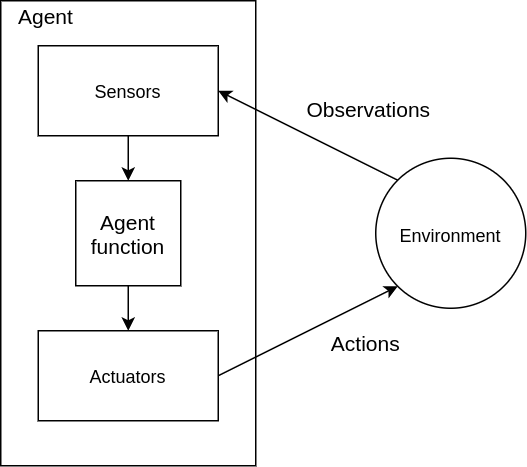
\includegraphics[height=7cm, keepaspectratio]{agent_environment_loop.png}
    \caption{The agent-environment interaction loop}
    \label{agent_environment_loop}
\end{figure}

\section{Environment}
Now that we have a general understanding for agents and environments, we can use this knowledge to have a closer look at Abalone. It is a fairly new game, that was devised in 1987 by Michel Lalet and Laurent Lévi. Nevertheless, with more than four million global sales it has established itself as a classic game \cite{noauthor_abalone_2020}. Abalone is a two-player game consisting of a hexagonal board with 61 fields and 14 marbles for black and white respectively.

\subsection{Abalone rules}
The goal of the game is to push six of the opponent's marbles off the playing field. The game's starting position is depicted in figure \ref{basics} (a). One, two, or three adjacent marbles (of the player's own color) may be moved in any of the six possible directions during a player's turn. We differentiate between broadside or "side-step" moves and "in-line" moves, depending on how the chain of marbles moves relative to its direction, which is shown in figure \ref{basics} (b) and (c).

\begin{figure}[!h]
    \centering
    \subfloat[Starting position]{
        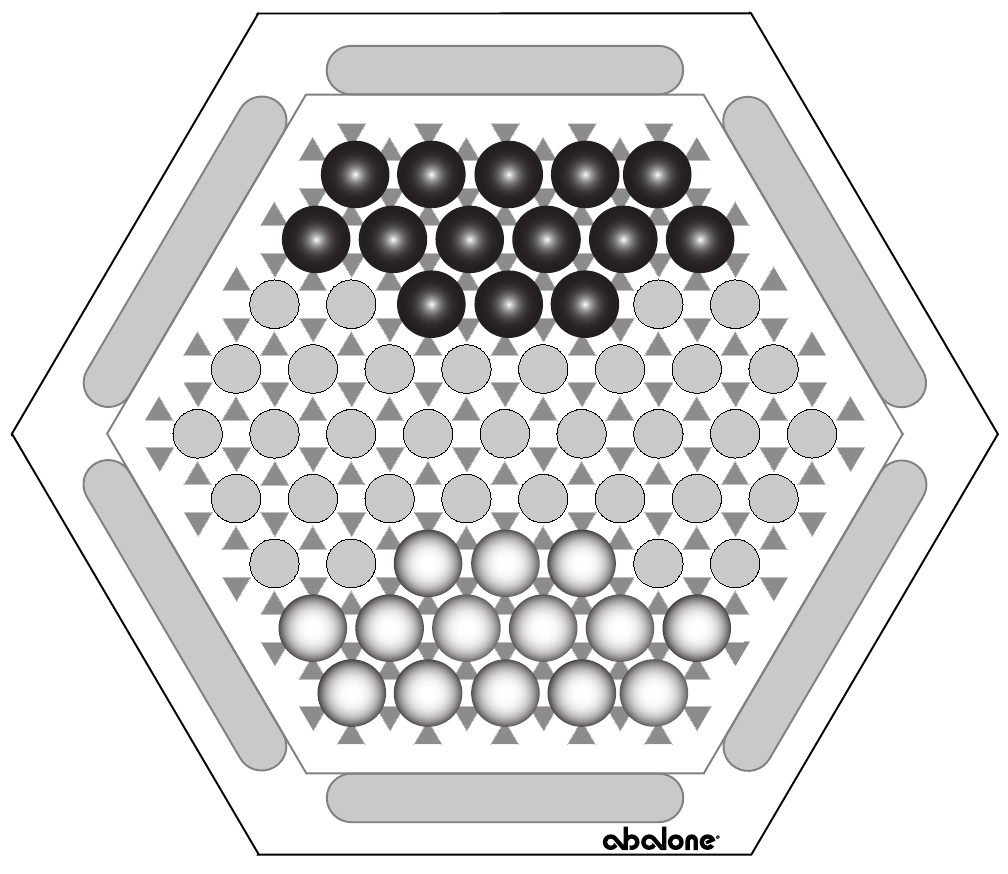
\includegraphics[width=3cm, keepaspectratio]{rules_starting_position.png}
    }
    \hfill
    \subfloat["In-line" moves]{
        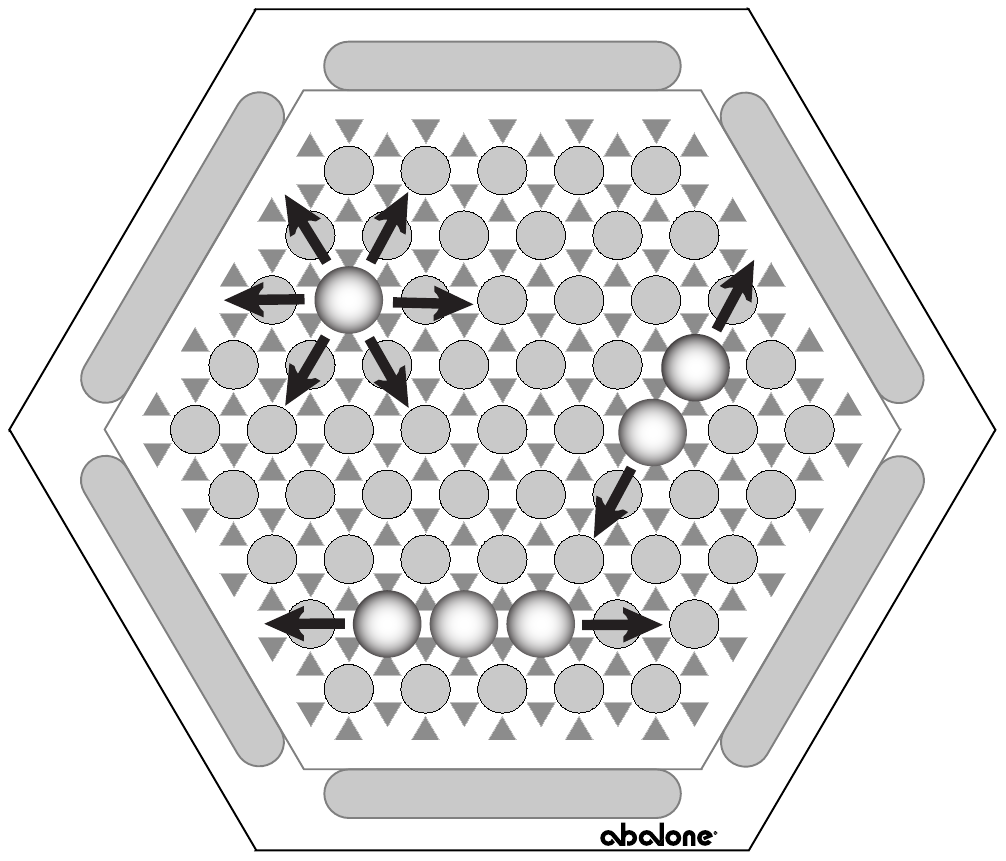
\includegraphics[width=3cm, keepaspectratio]{rules_inline_move.png}
    }
    \hfill
    \subfloat["Side-step" moves]{
        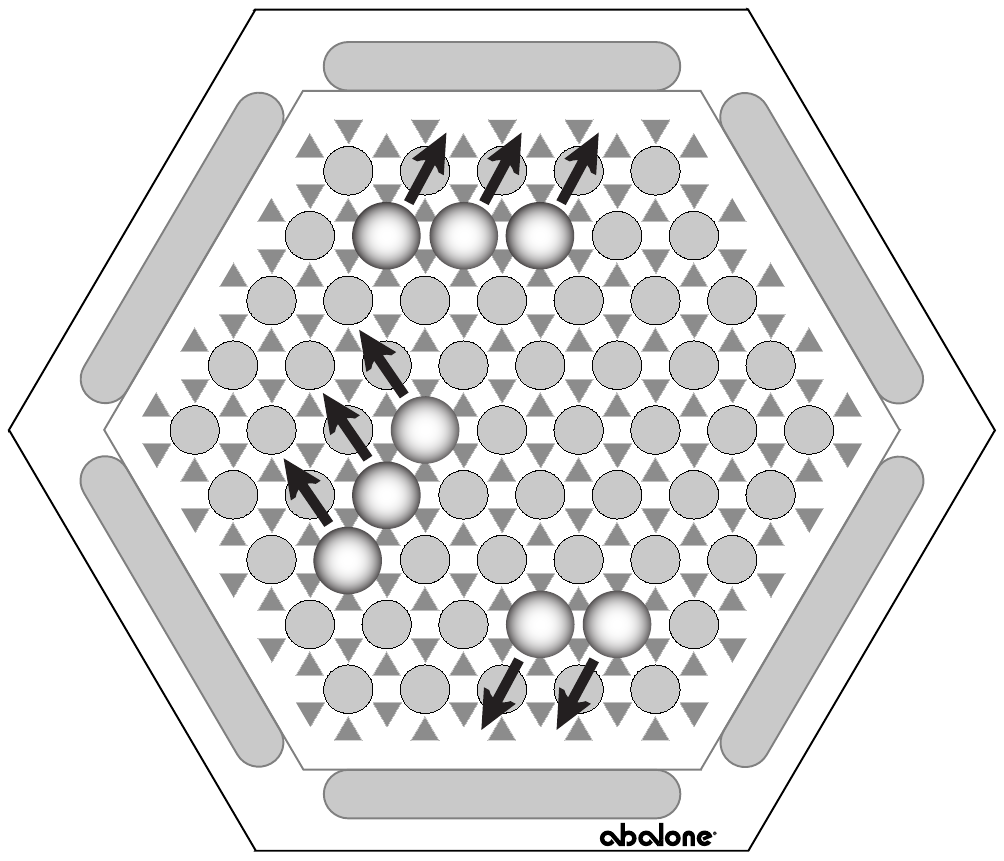
\includegraphics[width=3cm, keepaspectratio]{rules_side_step_move.png}
    }
    \caption{Basic moves \cite{abalone_sa_abalone_nodate}}
    \label{basics}
\end{figure}

A move pushing the opponent's marbles is called "sumito" and comes in three variations, as shown by figure \ref{sumito}. Essentially, the player has to push with superior numbers and the opponent's marbles can not be blocked. This is the game mechanic that allows for pushing the marbles out of the game and winning.

\begin{figure}[!h]
    \centering
    \subfloat["2-push-1" sumito]{
        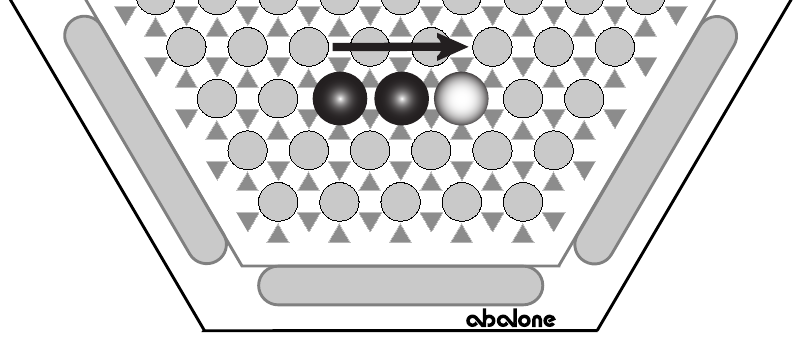
\includegraphics[width=3cm, keepaspectratio]{rules_2-push-1_sumito.png}
    }
    \hfill
    \subfloat["3-push-1" sumito]{
        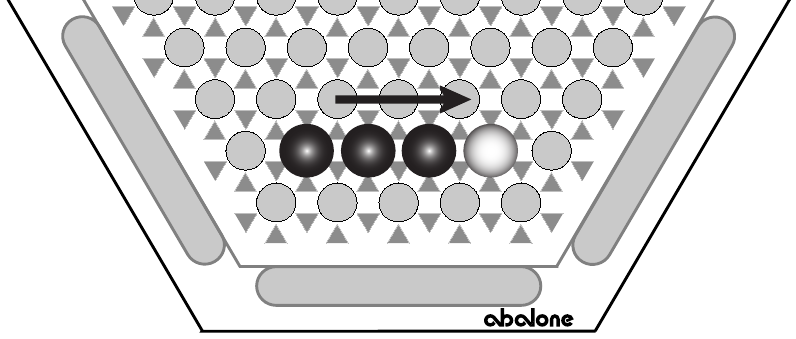
\includegraphics[width=3cm, keepaspectratio]{rules_3-push-1_sumito.png}
    }
    \hfill
    \subfloat["3-push-2" sumito]{
        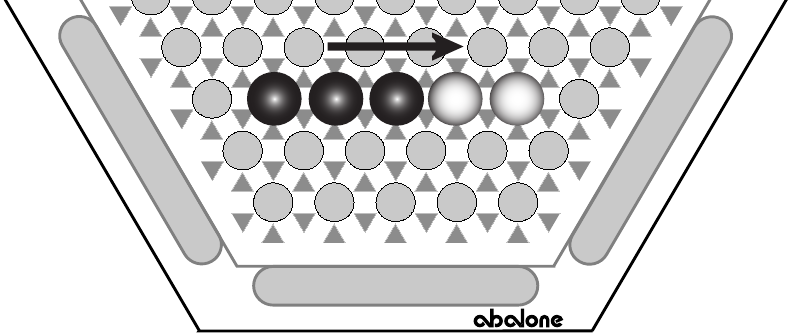
\includegraphics[width=3cm, keepaspectratio]{rules_3-push-2_sumito.png}
    }
    \caption{Sumito positions allow pushing the opponent's marbles \cite{abalone_sa_abalone_nodate}}
    \label{sumito}
\end{figure}

\subsection{PEAS and task properties}
Based on the PEAS framework we can specify Abalone as a task environment and show the key componentents for the implementation of our agent. \cite[p.107]{russell_artificial_2021}

\begin{description}
    \item[Performance measure] Win/loss, number of moves, time to deliberate
    \item[Environment] Digital playing board
    \item[Actuators] Move marbles, display text to CLI
    \item[Sensors] Position of marbles
\end{description}

There are a few categorizations that are extremely helpful for narrowing down potential applicability of different classes of algorithms. A key property is the observability of the environment. If the environment is \textit{fully observable}, the sensors detect all the information that is in any way relevant for taking an action. Conversly if not all information can be oberserved we call it \textit{partial observability}. For example in poker the other players' cards and the upcoming cards cannot be seen but are highly relevant to the agents actions. As the current board state of Abalone fully comprises all information necessary to make a move, we can classify it as fully observable.

The values the state of the environment and time can be categorized into discrete and continuous. The autonomous vehicle for instance is dealing with continous time and also continous states. The speeds of the car take a smooth range of real values and time can be meaningfully split into increasingly small intervals. However, Abalone is entirely discrete. The set of all states is a finite collection of all (legal) permutations of the board and the marbles. Time progresses on the basis of turns.

The actions that the agents takes might also be \textit{non-deterministic}. When dealing with systems of high complexity the next state might not only depend on the previous state and the action taken. There might be other car drivers taking unexpected actions or a comet hitting our car. In Abalone none of these issues arise as it is deterministic.

Further expanding on the passage of time we have to take into account if actions have consequences for future states. If each combination of perecpt and action is independent of each other we call it \textit{episodic} and \textit{sequential} otherwise. If we had to classify a production line of circuit boards as either defective or functional, it would be an episodic environment. The classification of an individual board does not matter for the next one. In the case of Abalone moves taken have long drawn out consequences for later stages of the game.

Another aspect of time is whether the environment changes while the agent takes time to deliberate on the next move. In a \textit{dynamic} environment like the autonomous vehicle operates in, the environment changes continously. In the time the car decides whether to right, to avoid collision with a wall, this decision might have already become obsolete. As any turn based game, Abalone is a \textit{static} environment, as the board only changes after a move is made.

Lastly, an additional dimension to consider is the number of agents involved. The classification of circuit boards only involves one agent whereas Abalone is a \textit{multi-agent} environment. We also have to distinguish whether those multiple agents compete for the performance measure. In Abalone the one players win is the other players loss. In contrast, the other vehicles apart from our autonomous vehicle all profit when it avoids a collision and vice versa. Therefore, they cooperate.

Summing this up \textbf{Abalone is a fully observable, deterministic, two-agent, competitive, sequential, static and discrete environment}. Another popular term for this type of environment is a \textit{perfect information zero-sum game}.

\subsection{Abalone complexity}

As Abalone has a finite amount of discrete states, we can make precise statements about its complexity, which can be described in two relevant dimensions.

\paragraph{State space complexity}
The state space is the set of all possible states the environment can be in.\cite[p. 150]{russell_artificial_2021} For Abalone this means we have to consider all possible board configurations with different numbers of marbles present. Additionally, we would have to remove duplicates that arise from the symmetries of the board. In the case of abalone we have 6 rotations and 6 axes we can mirror the board on. The following formula gives us a good upper bound:

$$
    \sum_{k=8}^{14}\sum_{m=9}^{14}\frac{61!}{k!(61-k)!}\times\frac{(61-k)!}{m!((61-k)-m)!}
$$

\paragraph{Game tree complexity} The game tree defines all transitions between board positions (nodes) through moves (edges). The \textit{search tree} is potentially a subset of the game tree, if not all paths are visited. In the case of Abalone the game tree is unbound and has an infinite height as actions might be taken repeatedly forming loops. To get a measure of the complexity the number of nodes in a tree is given by:

$$
    b^d
$$

First we consider the branching factor $ b $, or the number of possible moves for any given state. We can only approximate this, as this number greatly varies between different states. On average abalone has $ b = 60 $ possible moves per state as measured in figure \ref{branching_factor}. The depth $ d $ of the tree depends the number of turns per game. Looking at the average again a game takes in the region of $ d = 87 $ turns, giving us a total of $60^{87}$ nodes. To be precise this is the complexity of an average search tree not the game tree, as mentioned above. \cite{lemmens_constructing_2005}

\begin{figure}
    \centering
    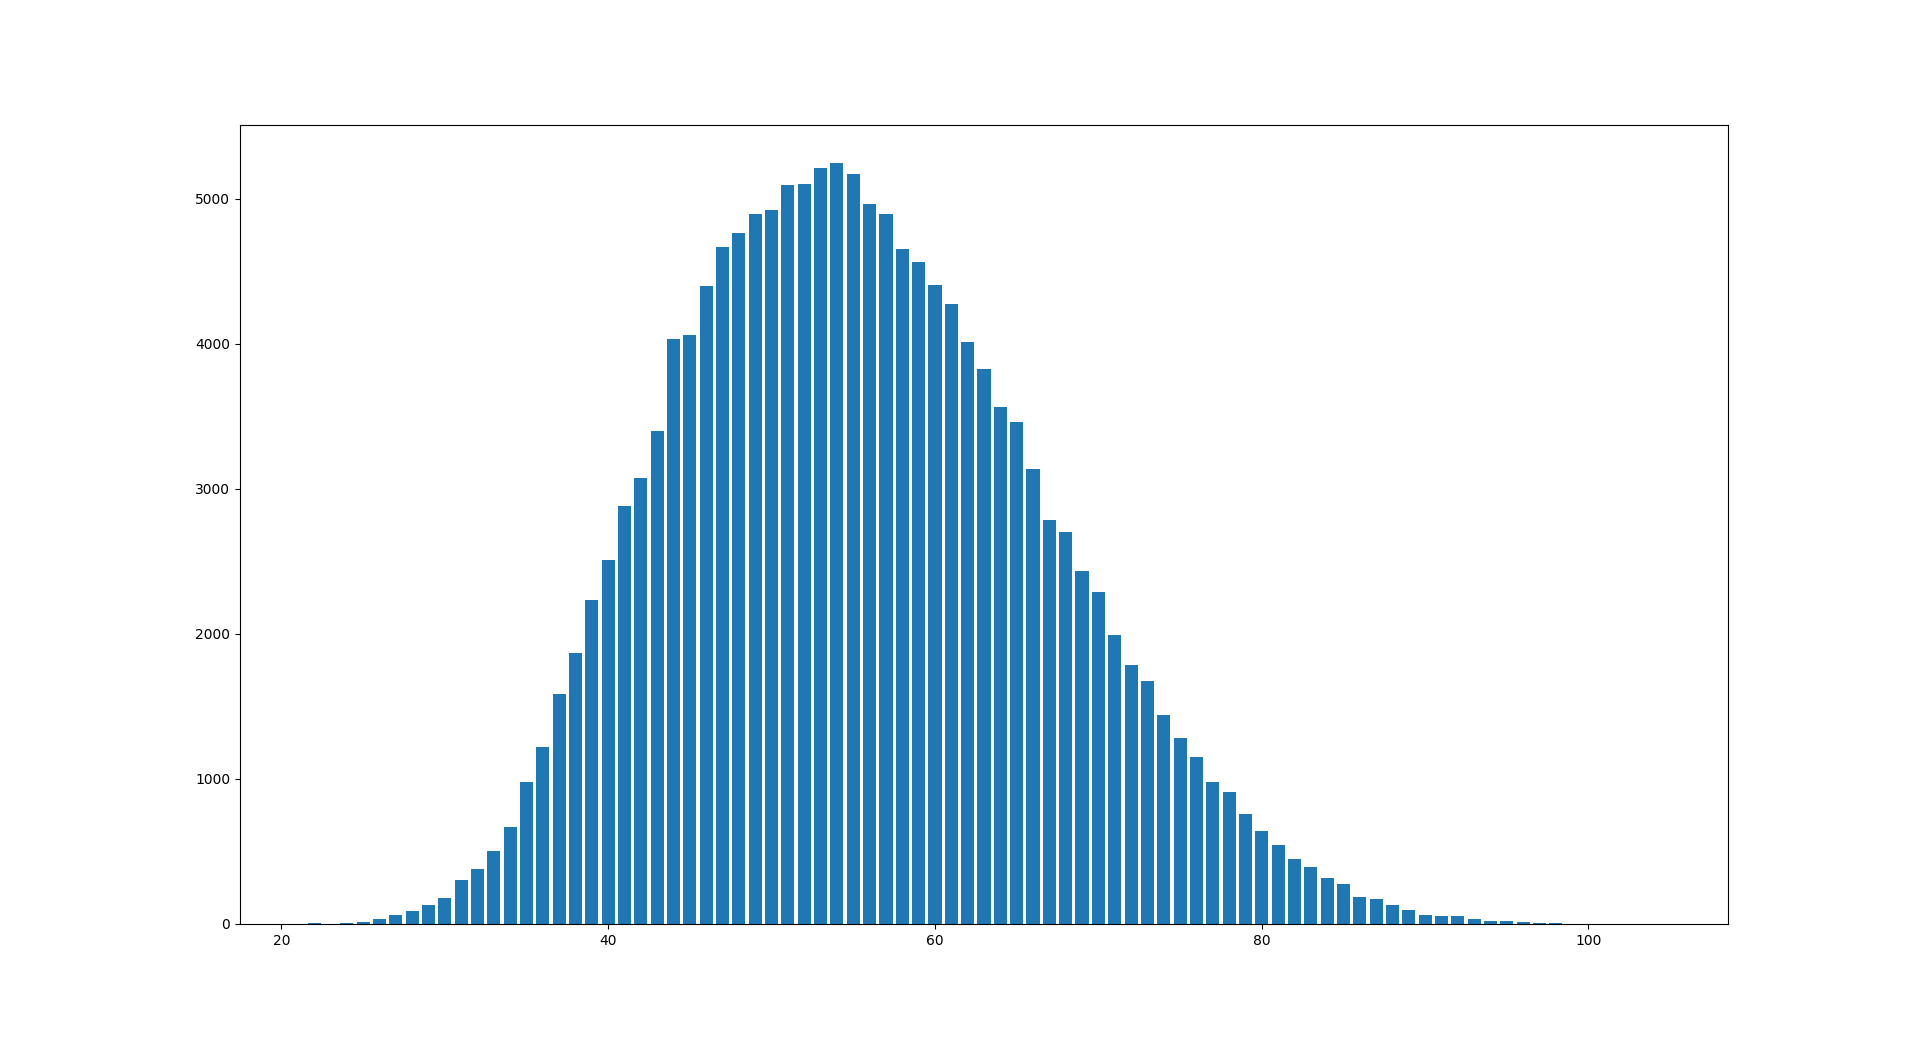
\includegraphics[width=7cm, keepaspectratio]{distribution_of_moves.png}
    \caption{Counts of moves available for random for random player in 5 games}
    \label{branching_factor}
\end{figure}

As those numbers in isolation are hard to grasp it is useful to put Abalone's complexity in relation with other popular games. Its state space complexity is on the same level as Reversi, whilst its game tree surpasses chess in complexity (c.f. table \ref{complexity_table})

\begin{table}
    \begin{center}
        \begin{tabular}{ | c | c | c | }
            \hline
            Game        & state-space complexity (log) & game-tree complexity (log) \\
            \hline
            Tic-tac-toe & 3                            & 5                          \\
            \hline
            Reversi     & 28                           & 58                         \\
            \hline
            Chess       & 46                           & 123                        \\
            \hline
            Abalone     & 24                           & 154                        \\
            \hline
            Go          & 172                          & 360                        \\
            \hline
        \end{tabular}
    \end{center}
    \caption{Abalone in comparison with other games \cite{chorus_implementing_2009}}
    \label{complexity_table}
\end{table}


\section{Classic agent}
Now that we have an intricate understanding of the environment for our agent we have also narrowed down the choice of algorithms we can employ. In general, perfect information games can be solved by adverserial search algorithms. That means in theory we can find the optimal solution by traversing the entire game tree to terminal states (game ending state). The theory behind this type of agent was already laid out as early as 1945 by Konrad Zuse's program generating legal chess moves \cite{knuth_early_1980}, but was described most comprehensively by Claude Shannon in 1950 in "rogramming a Computer for Playing Chess". \cite{shannon_xxii_1950}

\subsection{Minimax algorithm}
Minimax assumes two roles: The minimizer and the maximizer. We start the search from the current board state as the role of the maximizer and then alternate between the two. The result of the minimax search gives us the maximum utility for the given state, assuming both players behave optimally. Let us define the functions
\begin{itemize}
    \item $\text{utility(s, p)}$ returns the utility or the payoff for the terminal state $s$ seen from the perspective of player $p$. In the case of abalone this might be -1, 0 and 1 for a loss, draw and a win.
    \item $\text{is-terminal(s)}$ returns whether the given state $s$ is a terminal state or not
    \item $\text{to-move}(s)$ returns the current player for the state $s$
    \item $\text{result}(s, a)$ returns the resulting state if in state $s$ and taking action $a$
\end{itemize}
such that we can define minimax recursively as:
$$
    \text{minimax}(s) =
    \begin{cases}
        \text{utility}(s, max)                                                & \text{is-terminal}(s)    \\
        \text{max}_{a\in\text{actions}(s)}\text{minimax}(\text{result}(s, a)) & \text{to-move}(s) == max \\
        \text{min}_{a\in\text{actions}(s)}\text{minimax}(\text{result}(s, a)) & \text{to-move}(s) == min \\
    \end{cases}
$$

Putting this together we can see in figure \ref{minimax} a graphical representation of the search tree for an abstract example. The algorithm traverses down to a leaf node, evaluates its utility and passes the value back up to the parent node. Depending on whether it is a minimizer or a maximizer it chooses the smallest or the largest value passed up its children. This value again is passed up to the parent until we reach the parent node which is always a maximizer, yielding us the maximum utility we can achieve given our opponent plays optimally.

\begin{figure}
    \centering
    % \includesvg[height=7cm]{minimax.svg}
    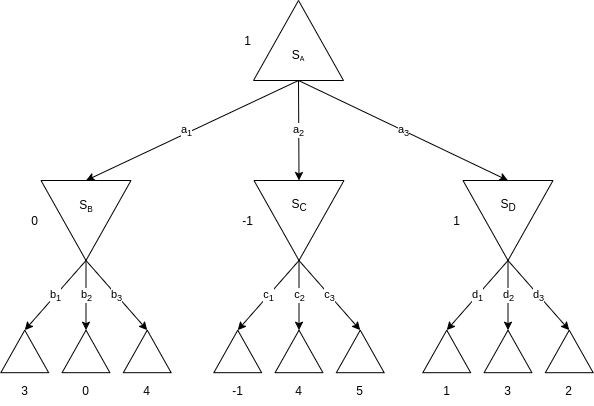
\includegraphics[height=7cm, keepaspectratio]{minimax.png}
    \caption{Minimax for a small search tree, resulting in an utility value of 1}
    \label{minimax}
\end{figure}

\subsection{Heuristic functions}
As the number of nodes of the game tree gets very large, the search on the tree usually does not reach terminal leaves that indicate a clear loss or win. Our computational resources will get exhausted first. For example minimax has already visited $ 60 ^ 4 = 1.2960.000 $ nodes at a depth of $ d = 4 $ in the case of an average Abalone game.

Therefore, one has to limit the search to a computationally feasable depth and evaluate the intermediary result of a given transposition based on a so called \textit{heuristic function}. This function replaces our previous $ utility(s) $ for terminal states and is based on human knowledge. The function should give a precise feedback, on the quality of a state from the perspective of the given player. A sensible function for Abalone might be a linear combination in the form of:

$ h(s) = \omega_0f_0(s) + ... + \omega_nf_n(s) $

With functions $ f_i $ calculating different values such as

\begin{itemize}
    \item Adjacency: As a majority of marbles is required to push opponent's marbles and conversely an equal amount of marbles is needed to avoid being pushed, it can be assumed that keeping one's marbles grouped together is a good move.
    \item Distance to center: Marbles that are close to the brink of the board put them into danger of being attacked, wherefore it is generally good to place all of the marbles into the center of the board. For each player's marbles we measure their distance from the center of the board as the smallest amount of moves it would take to reach the center (Manhattan distance).
    \item Win and loss: As a more definitive measure we can indicate whether the current state is a terminal state and hence a winning or losing state.
    \item Etc.
\end{itemize}

By applying different weights $ \omega_i $ to the functions $ f_i $ we essentially give incentives to the agent to prioritize certain behavior. If the win or loss function returns a value of either -1 or +1, we might combine it with a weight of 10.000 to make sure we choose winning states and avoid losing states above all. Armed with this heuristic function we can find good moves with minimax search even in highly complex state spaces.

However, the problem with heuristic is we need expert knowledge and a lot of empirical testing to find a suitable heuristic. In some cases like with Go, such a heuristic function might not be competitive with even moderate human players. In other cases such as chess this strategy is very powerful. As mentioned in the introduction IBM's Deep Blue could beat the world's best player Gary Kasparov based this heuristic based adverserial search.

\subsection{Alpha-beta pruning}
We can further improve minimax search markedly by using Alpha-beta-pruning. This method tries to eliminate unnecessary traversals down the search tree. In the best case, this leads to a reduction of nodes from $ O(b^d) $ to $ O(\sqrt{b^d}) $.

\begin{figure}
    \centering
    % \includesvg[height=7cm]{alpha_beta_pruning.svg}
    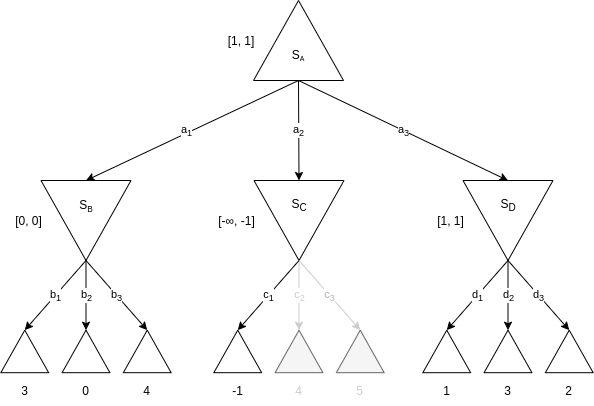
\includegraphics[height=7cm, keepaspectratio]{alpha_beta_pruning.png}
    \caption{Our previous example but with alpha beta pruning applied. The greyed out nodes indicate, that these in fact could be pruned from the tree}
    \label{alpha_beta_pruning}
\end{figure}

The order in which we visit nodes in minimax is similar to a graph traversal with depth first search, meaning we descend down until we find a leaf node. This gives us information about the utility of that node and, consequently, part of the tree. Going up the tree we keep an alpha value for the minimum value the maximizer will recieve and a beta value for the maximum value the minimizer will achieve. For instance this lets us know if the minimizer already can choose a move worse than what we can achieve with another move, we not descend further $ (\alpha > \beta) $.

Looking at the example in figure \ref{alpha_beta_pruning} will help us illustrate this principle. Our search revealed that choosing move $ a_1 $ will yield us an utility of at least 0. Traversing down move $ a_2 $ the first leaf has a utility of -1. Hence, the minimizer will choose a move that is at most -1 which is already worse than the utility of 0. We need not look further at this part of the tree.

The example also shows us a important prerequisite for this method to work. The order in which we expand which node matters decides how much nodes we can prune. Had we visited move $ c_3 $ and $ c_2 $ first, pruning wouldn't have been possible. The best case of $ O(\sqrt{b^d}) $ is entirely dependent on this ordering. We could find different ways of ranking the moves:

\begin{itemize}
    \item \textit{Killer move heuristic} prioritizes that are usually undoubtedly good like taking a marble in Abalone.
    \item \textit{Iterative deepening} Performs a minimax search only to a depth of one and uses the resulting values to rank the moves. Then searching one level deeper we use this ranking for ordering the moves. Even though there is a lot of redunancy, we make up for this more than enough by pruning much more effectively.
\end{itemize}

Other improvements to the procedure are thinkable as well. Once we performed a search for a certain state, we can store the resulting utility. If we encounter this position again, because of a different permutation of the move sequence (transposition), we can just look up the state utility in the \textit{transposition table}.

Combined with alpha beta pruning, the minimax algorithm is a very efficient way of finding the optimal utility in an adverserial search situation. However, as mentioned before in most games we cannot use the utility of terminal states, because the search tree grows too quickly. By optimizing for a heuristic function the quality of play solely depends on this function. For games such as Chess or Abalone minimax has been very successful, because humans could devise meaningful heuristic functions. For chess the engine stockfish has been the most successful computer player for a long time and is based on this algorithm (and many optimizations). \cite{noauthor_stockfish_2021, noauthor_stockfish_nodate} In Abalone there are multiple implementations, the most successful has been ABA-PRO by Tino Werner \cite{aichholzer_algorithmic_2002} which has been the reference for other algorithms such as Abalearn \cite{campos_abalearn_2003}. A more recent publication claimed more successful play \cite{papadopoulos_exploring_2012} which was comfirmed in a very recent reimplementation thesis \cite{verloop_critical_nodate}. This reimplementation in Java \cite{verloop_abaloneai_nodate} is also the reference for later benchmarks.

\subsection{Monte Carlo Tree Search}
For games like Go we cannot find powerful heuristic functions, which makes the previous approach of minimax not a viable option. In addition, the initial position of a 19x19 Go boarad is 361 decreasing only by one for each stone placed. A method proposed in 2006 by Coulom \cite{coulom_efficient_2007} called Monte Carlo Tree search. The main idea is to use simulations or \textit{rollouts} to gain information on the quality of a state. To manage the complexity of the search tree more effectively the algorithm is \textit{selective} in which parts of the tree are \textit{expanded}. This ensures that resources are not wasted on unpromising moves.

In its purest form the simulations are performed randomly, meaning we take state or node to be investigated and let two random players take turns until a terminal state is reached. Kocsis and Szepesvári \cite{kocsis_bandit_2006} showed that is in fact does converge to optimal play. For games like Abalone with high branching factor we need a large number of simulations to get any meaningful information from the simulations, so we might use a \textit{rollout policy} instead. This policy guides the moves taken in the simulation towards better moves. This might be as simple as favoring capturing moves or as we will see later neural networks.

The algorithm can be structured into four stages:

\paragraph{Selection} is the process of deciding which node to consider next. We start at the root node and select a node until we reach a leaf node. This is the secleted Node. We could select the nodes according to some stationary distribution or we could use the information that we gain over time.

\paragraph{Expansion} is the step in which we expand the selected node by appending a fresh child node.

\paragraph{Simulation} is as described as before the step in which we perform a simulation with our rollout policy starting from the state of the newly generated child node.

\paragraph{Back-propagation} is the last step. We take the result of the simulation (utility) and write it to the node and parent nodes above until we reach the root node. Each node updates its cumulative utility $U(n)$ and the number of times it was visited $N(n)$.

The more we repeated this cycle, the more certainty we gain about the optimal move to take.

\begin{figure}
    \centering
    % \includesvg[height=7cm]{minimax.svg}
    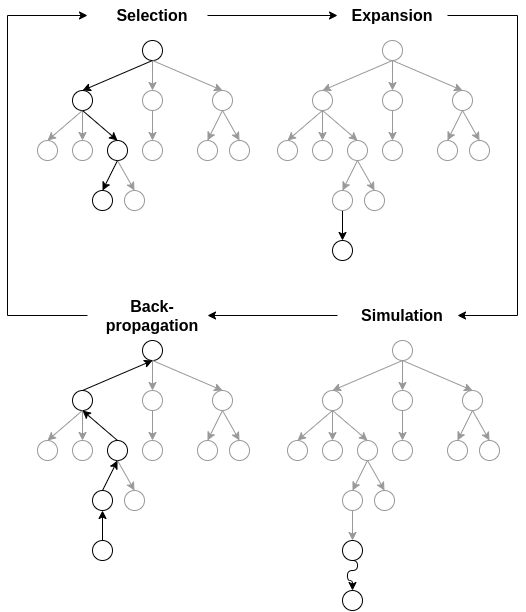
\includegraphics[height=9cm, keepaspectratio]{monte_carlo_tree_search.png}
    \caption{Monte Carlo tree search stages \cite{noauthor_fig_nodate}}
    \label{monte_carlo_tree_search}
\end{figure}

The inception on MCTS led to significant improvements in performance of game-playing agents in the Game of Go. The algorithm "Crazy Stone" from Coulom won the 10th KGS computer-Go tournament against competitors such as Indigo \cite{bouzy_associating_2006}. To select the next node he estimated the probability that move being better than the current best move. We order the moves by their current estimated value $ \mu_i $ and calculate the corresponding variance $ \sigma_{i}^{2} $ getting the ordering of $ \mu_0 > \mu_1 > ... > \mu_N $. Selection of a move is proportional to:

$$
    u_i = exp\left(-2.4\frac{\mu_0 - \mu_i}{\sqrt{2(\sigma_{0}^{2} + \sigma_{i}^{2})}}\right) + \epsilon_i
$$

The Term $ \epsilon_i $ ensures that the probability of selection never goes to zero as defined by $ \epsilon_i = \frac{0.1 + 2^{-i} + a_i}{N} $. The resulting distribution is similar to the Gaussian distribution and the Boltzman equations \cite{coulom_efficient_2007}

Another idea for selection is the UCB1 formula \cite{auer_finite-time_nodate}, that weights how often we have visited a node and how promising it is.

$$
    \text{UCB1}(n) = \frac{U(n)}{N(n)} + C \times \sqrt{\frac{\log{N(Parent(n))}}{N(n)}}
$$

The cumulative utility $U(n)$ is normalized by the number of times we have visited the node $N(u)$. This helps favoring moves that are either relatively unexplored and promising or have proven to be good over a larger set of nodes. It is also called the exploitation term. The additional term is called the exploitation term. The more often we visit a node, the smaller this term gets, converging to 0 for large $N(n)$. The constant factor $C$ is subject to some debate which value might be optimal, some choose $\sqrt{2}$. In general, this hints at another point of investigation: The problem of \textit{explotation vs. exploitation} \ref{exploration_vs_exploitation} that we will inspect more closely later.

Here we can already see David Silver's handwriting on the wall. As early as 2006 he, and Sylvian Gelly, investigated optimization to MCTS \cite{gelly_achieving_nodate} for the game of Go. In 2011 they published a comprehensive paper \cite{gelly_monte-carlo_2011} proposing the algorithm MoGo and evaluating different strategies to improve the effectiveness of MCTS in Go. Seeing that

\begin{quotation}
    [...] professional Go players often play moves according to intuitive feelings that are hard to express or quantify. Precisely encoding their knowledge into machine-understandable rules has proven to be a dead-end: a classic example of the knowledge acquisition bottleneck.
\end{quotation}

One of the ideas introduced is Rapid Action Value Estimation (RAVE). We already saw how we could reuse information gathered for minimax through a transposition table. In our search tree we will encounter transpostions for that we already performed searches. RAVE allows us to reuse experience gathered from simulations for related positions. A key property observed by Silver was that MoGo scales proportional to the amount of compute or rather number of simulations it can perform per turn as depicted in figure \ref{mogo_scaling}.


\begin{figure}
    \centering
    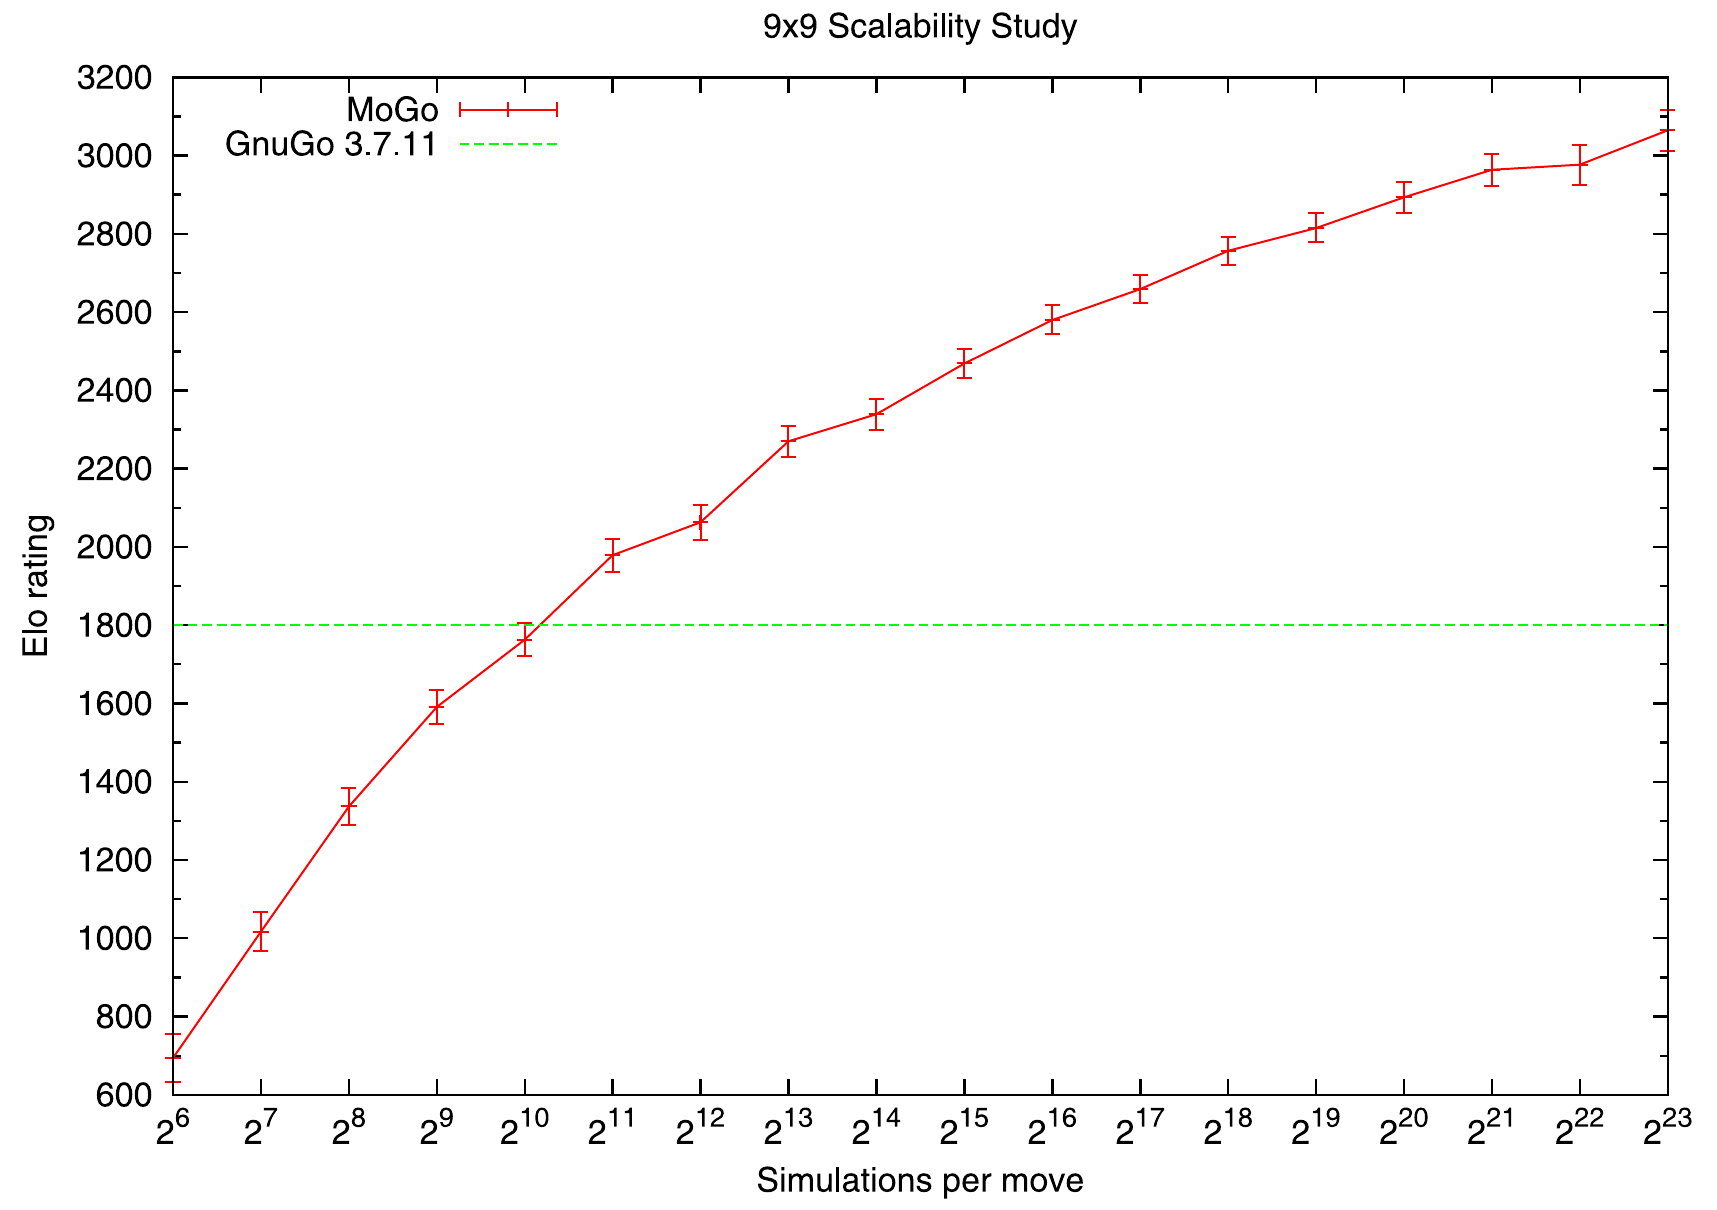
\includegraphics[height=7cm, keepaspectratio]{mogo_scaling.png}
    \caption{Elo rating of MoGo in relation to the computational resources granted to the algorithm \cite{gelly_monte-carlo_2011}}
    \label{mogo_scaling}
\end{figure}



\section{Learning agent}

\subsection{Markov decision process}

\subsection{Reinforcement learning}

\subsection{Exploration vs. Exploitation}
\label{exploration_vs_exploitation}
\chapter{System Architecture}
\label{system-architecture}
Well equipped with all the essential theoretical tools that we need, we can move on to implementing them for the game of Abalone. The first logical step would be to look at the existing software landscape to decide if we can utilize existing tools to speed up development.

\section{Software}
\subsection{Deep Learning Library}
Deep learning projects share many components. Most commonly, that is the declaration of the computational graph and the training of the graph. The libraries provide those components and bring significant optimizations and specialized code for hardware acceleration. Therefore, it is imperative to decide on a suitable library to speed up development by several orders of magnitude.

\begin{figure}
    \centering
    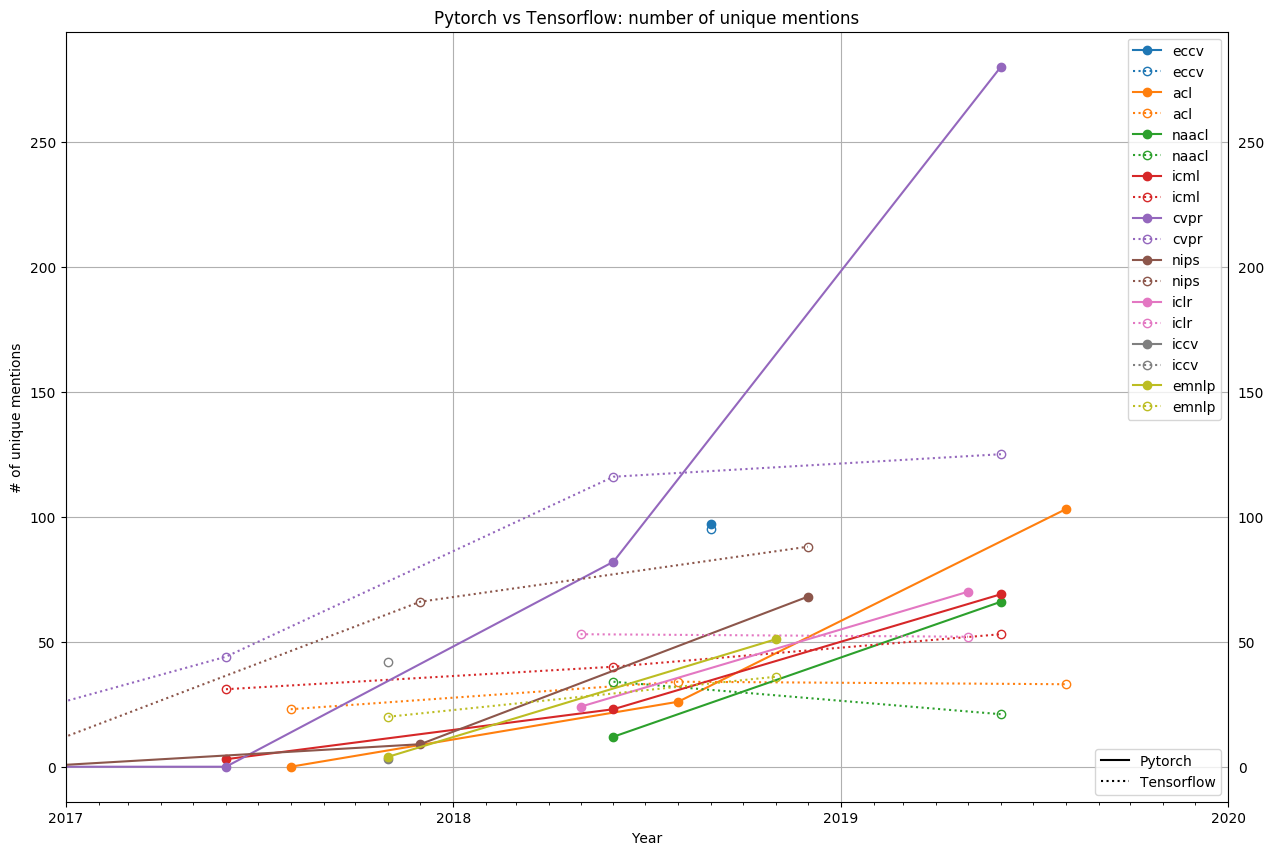
\includegraphics[height=7cm, keepaspectratio]{ml_framework_popularity.png}
    \caption{The mentions of PyTorch and tensorflow in research papers in different publications \cite{noauthor_state_2019}}
    \label{ml_framework_popularity}
\end{figure}

The first indicator to go by is the popularity of the frameworks. The most relevant frameworks are Facebook's PyTorch and Google's TensorFlow. The Keras API has been introduced to TensorFlow, wherefore it is not considered further. In research, PyTorch seems to have quickly taken the dominance as depicted in figure \ref{ml_framework_popularity}. Aside from all differences between both libraries, the choice was guided by two practical reasons. Initially, we selected TensorFlow due to the included support for TPUs as Google granted this project free access to their Research Cloud \cite{noauthor_tpu_nodate}. At a later stage, it became clear that Google was unwilling to increase the CPU quota for the account, limiting the server to 8 cores which posed a significant problem for parallel execution.

In table \ref{pytorch_vs_tensorflow_performance} there is also a significant performance difference in the inference step of the MCTS. There are two ways in TensorFlow to perform inference, either through the \texttt{predict} function or by calling the \texttt{\_\_call\_\_} method of the $model$ itself. As in the implementation, the inference is not batched but done for individual board states. The usage of the latter option is faster \cite{noauthor_tfkerasmodel_nodate}. Nevertheless, PyTorch is about five times faster. As discussed later, this is the reason to pivot to PyTorch as a framework.

\begin{table*}
    \begin{center}
        \begin{tabular}{ c|c|c|c|c }
            HW  & Framework & Neural net size & $\texttt{predict}(s)$ & $\texttt{\_\_call\_\_}(s)$ \\
            \hline
            \hline
            CPU & tf        & small           & ~0.027s               & ~0.011s                    \\
            GPU & tf        & small           & ~0.024s               & ~0.005s                    \\
            CPU & tf        & large           & ~0.027s               & ~0.015s                    \\
            GPU & tf        & large           & ~0.025s               & ~0.011s                    \\
        \end{tabular}
    \end{center}
    \caption{The average time ($n = 3,000$) taken to perform the feed-forward through the network for state $s$ with either ($\texttt{predict}(s)$) or ($\texttt{\_\_call\_\_}(s)$) in tensorflow}\label{tensorflow_predict_vs_call}
\end{table*}

\begin{table*}
    \begin{center}
        \begin{tabular}{ c|c|c|c|c }
            HW  & Framework & Neural net size & $\texttt{predict}(s)$ & $\texttt{search}(s)$ \\
            \hline
            \hline
            CPU & tf        & small           & ~0.01s                & ~0.016s              \\
            GPU & tf        & small           & ~0.005s               & ~0.011s              \\
            CPU & tf        & large           & ~0.014s               & ~0.02s               \\
            GPU & tf        & large           & ~0.011s               & ~0.017s              \\
            CPU & PyTorch   & small           & ~0.005s               & ~0.011s              \\
            GPU & PyTorch   & small           & ~0.001s               & ~0.007s              \\
            CPU & PyTorch   & large           & ~0.005s               & ~0.011s              \\
            GPU & PyTorch   & large           & ~0.002s               & ~0.008s              \\
        \end{tabular}
    \end{center}
    \caption{The average time ($n = 3,000$) taken to perform the feed-forward through the network for state $s$ ($\texttt{predict}(s)$) and one iteration of MCTS ($\texttt{search}(s)$)}\label{pytorch_vs_tensorflow_performance}
\end{table*}

\subsection{Training Framework}
\label{training_framework}
As there are existing frameworks that have implemented the system described in the AlphaZero paper in a more general and adaptable fashion, it has to be considered building on their foundation:
\begin{itemize}
    \item AlphaZero General is a framework developed as a university project at Stanford originally for the game of Hex and Othello. \cite{thakoor_learning_nodate,thakoor_suragnairalpha-zero-general_nodate}.
    \item Deep MCTS is a framework developed in the context of a Master's thesis \cite{bruasdal_deep_2020,henribru_deep_2021}.
\end{itemize}

We considered a catalog of criteria to compare both options. Parallel training and parallel search measure whether the software implements the parallel training pipeline and MCTS-APV proposed by the AlphaZero paper. Moreover, we checked whether the libraries are agnostic to the game and ML library. Lastly, it is relevant to investigate whether other users could verify the performance.

\begin{table*}
    \begin{center}
        \begin{tabular}{ c|c|c }
            Criterion             & AlphaZero General & Deep MCTS \\
            \hline
            \hline
            Parallel training     & 0                 & 1         \\
            Parallel search       & 0                 & 0         \\
            ML library agnostic   & 1                 & 0         \\
            Game library agnostic & 1                 & 1         \\
            Verified performance  & 1                 & 0         \\
            Simplicity            & 1                 & 0         \\
            \hline
            \hline
            Sum                   & 4                 & 2         \\
        \end{tabular}
    \end{center}
    \caption{A comparison of existing AlphaZero frameworks}\label{training_framework_comparison}
\end{table*}

As shown by table \ref{training_framework_comparison}, the winner by those criteria is AlphaZero General. The core advantages of the library are its simplicity and popularity. Deep MCTS makes use of a lot of abstractions and generics, which makes the code more professional and reusable. Nevertheless, this also poses significant difficulties in understanding. The application of AlphaZero General to multiple other games like Gobang, Santorini, Connect4, and more has shown its performance. The major drawback is the lack of a parallelized training pipeline.

\subsection{Game Engine}
There are multiple relevant implementations of game engines for Abalone. As the interfacing language for PyTorch is Python, it makes sense to restrict the engines to Python:

\begin{itemize}
    \item Abalone-BoAI is a game engine specifically designed for interfacing with computational agents. It is straightforward and has been used for the precursor project of this thesis \cite{scriptim_scriptimabalone-boai_2021}.
    \item Gym-abalone is tightly integrated with OpenAI's gym, potentially allowing agents to play other games as well. The API is suited for the reinforcement learning setting \cite{towzeur_towzeurgym-abalone_2021}.
\end{itemize}

Two arguments lead to the decision of choosing Abalone-BOAI:
\begin{enumerate}
    \item We already optimized it in the previous project, like the generation of legal moves.
    \item AlphaZero General expects the game engine to be designed in a functional way. The API of the engine needs to be adapted to fit the interface of the training framework. Both engines are stateful, meaning that they rely on the class instance context to perform moves, check for legal moves, and other operations. For instance, the operations are supposed to be applied to the input matrix, and the modified matrix is then returned. Therefore, intricate knowledge of the engine is of advantage.
\end{enumerate}

Due to those necessary modifications, we forked the original game engine to allow for more accessible packaging \cite{campfireman_campfiremanabalone-boai_2021}.

\begin{figure}
    \centering
    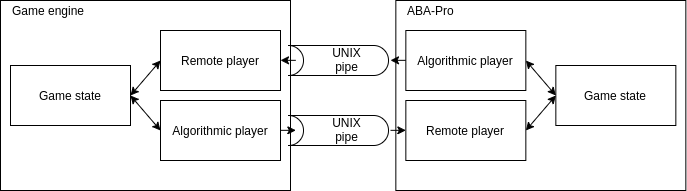
\includegraphics[height=4cm, keepaspectratio]{game_engine_communication.png}
    \caption{The inter process communication between the python game engine and the Java implementation of ABA-PRO}
    \label{python_java_ipc}
\end{figure}

As mentioned in the section \ref{existing_game_playing_agents}, Verloop's reimplementation \cite{verloop_abaloneai_nodate} offers the simplest solution for interfacing with (one of) the strongest Abalone algorithms. In a small tournament, personal implementations of minimax in Python \cite{claussen_abalone_2021} were inferior. As the Java implementation is tightly coupled with the internal game engine, we decided to implement a proxy player for each game engine. Each engine is a separate process, and the proxy players relay the moves between the engines. The proxy players communicate through a named pipe as depicted in figure \ref{python_java_ipc}. The downside of this solution is the need to synchronize two separate game states and translate between the different move notations. We used the notation introduced in section \ref{abalone_move_notation} to serialize the moves.


\section{Neural Network}
\subsection{Dimensions}
In order to apply the neural network architecture proposed by AlphaZero (cf. figure \ref{alpha_zero_neural_network}), two dimensions need to be changed:
\begin{enumerate}
    \item The input matrix of size $19 \cdot 19 \cdot 17$ needs to be adjusted to fit the dimensions of the hexagonal board. The hexagonal board is transformed into an orthogonal base as shown in \ref{abalone_matrix_representation} such that it can be represented as a $9 \cdot 9$ matrix.
          The third dimension of size $17$ can be reduced to 1 by removing the move history and only passing the current state. By representing the state as proposed in \ref{board_representations}, there are no separate planes necessary. Additionally, the board is always passed in its canonical form to the network. The board states are always seen from black's perspective in the canonical form. If it is the black player's turn, the board remains unchanged. If it is white's turn, the board's colors are switched. From the perspective of the neural network, white ($-1$) is always the opponent. The in-turn player is represented as $1$ and $-1$ for black and white. The matrix values can be multiplied with the in-turn player value to create the canonical form.
    \item AlphaZero's output vector $\pi$ of size 381 represents all possible positions a piece can be placed on the board. As Abalone has a much more complex move system, the size of this vector needs to match the number of all possible moves. We found the number of all possible moves by generating all moves programmatically. The generated moves were stored in a bijective map. Each move is assigned an index in $\pi$ and represented as a string in the proposed notation above. Therefore, using the bijective map, a move's index can be found by its string representation and vice versa.

          As depicted in figure \ref{possible_move_generation_inline}, the inline moves are generated by iterating over all fields of the board. For each field, all directions are tested for being a valid move. If that is the case, the move is added to the bijective map. In case the move is already present in the map, the move is skipped.

          \begin{figure}
              \centering
              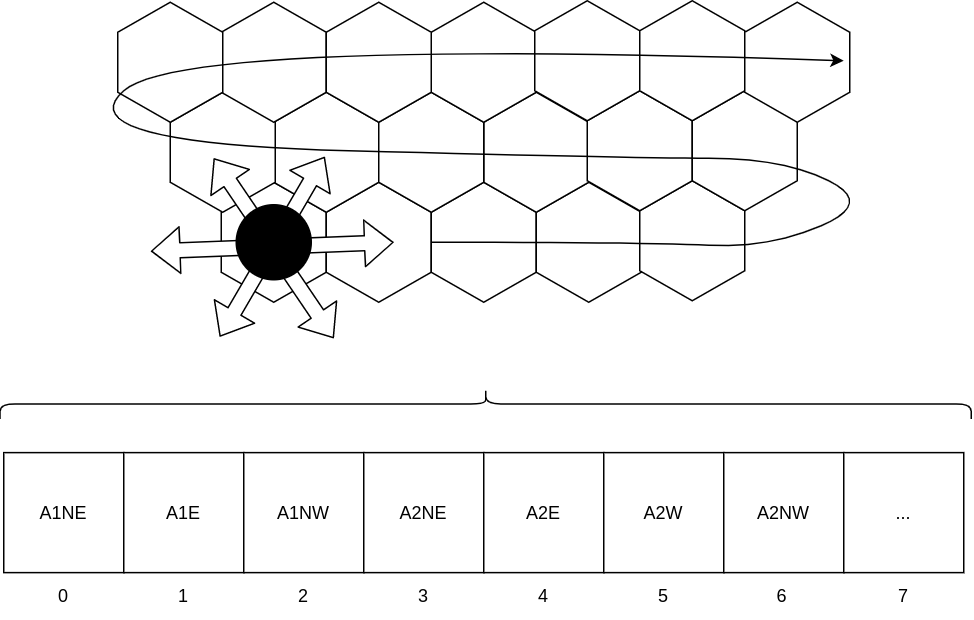
\includegraphics[width=12cm, keepaspectratio]{possible_move_generation_inline.png}
              \caption{Generation of inline moves, starting at position A1 and direction NE}
              \label{possible_move_generation_inline}
          \end{figure}

          Figure \ref{possible_move_generation_broadside} shows the generation of the broadside moves. The algorithm iterates each field. Marble lines of length two and three are generated in all (possible) directions for each field. For each line broadside in all directions, moves are checked for validity. The move direction of the marble line direction is ignored.

          \begin{figure}
              \centering
              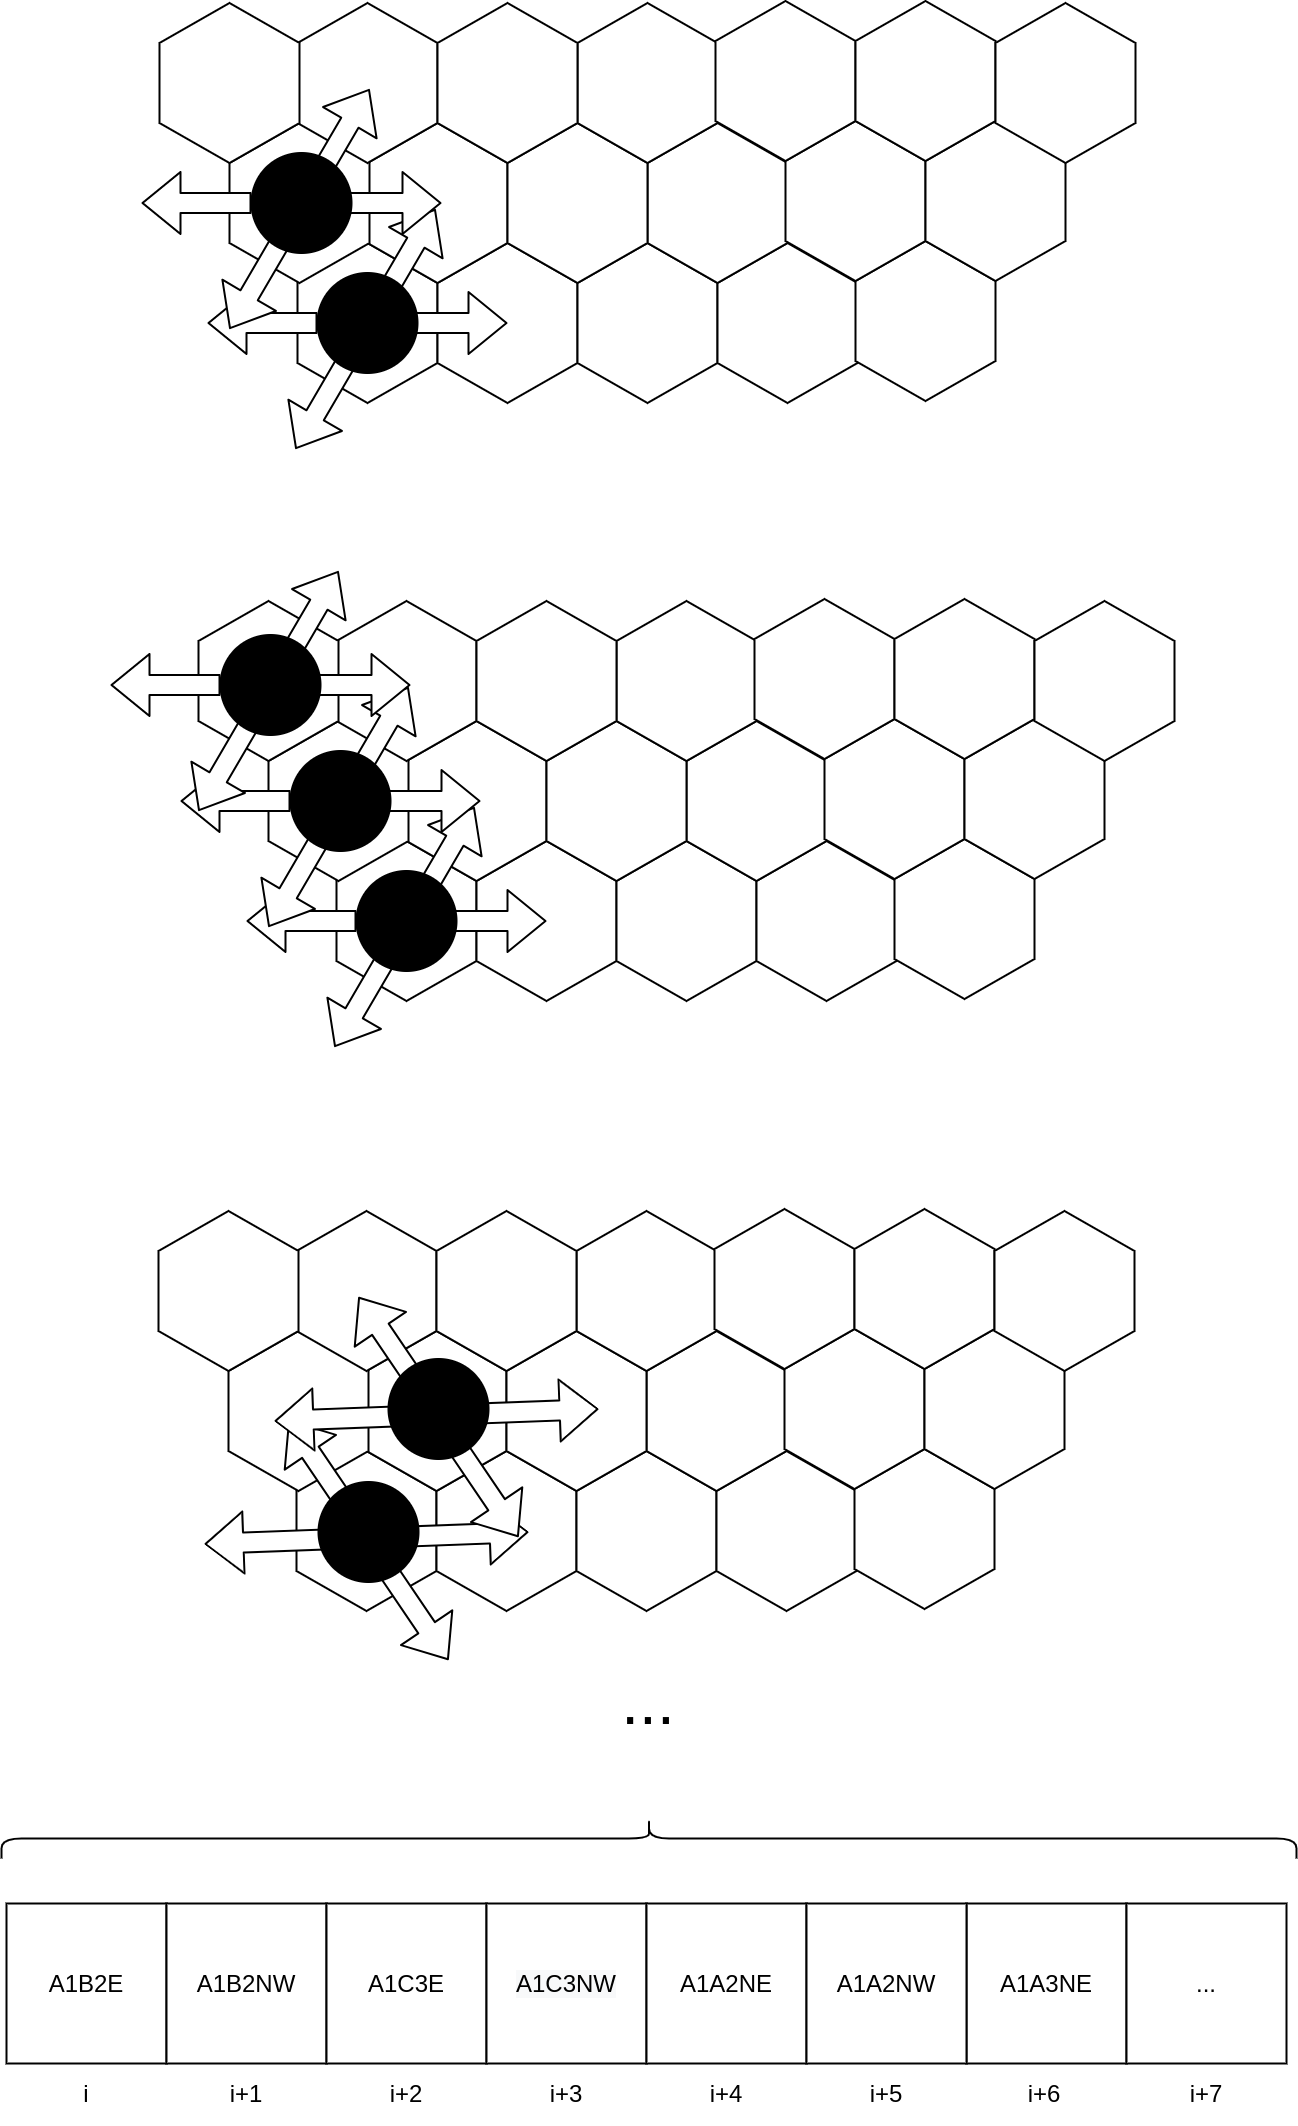
\includegraphics[width=12cm, keepaspectratio]{possible_move_generation_broadside.png}
              \caption{Generation of broadside moves starting at position A1, line direction NE, line length of two and at move direction NE}
              \label{possible_move_generation_broadside}
          \end{figure}

          The resulting vector $\pi$ has a length of $1452$.
\end{enumerate}

\subsection{Architecture}
\label{neural_network_architecture}
% explain pi and v
\section{Training Pipeline}
\subsection{Components}
\label{components}

The training pipeline of AlphaZero General has five main components:
\begin{enumerate}
    \item \textbf{Coach}: The main module that orchestrates the training process.
    \item \textbf{Game}: Provides an abstract interface that generalizes to many types of board games. Functions like the generation of legal moves, creating a unique string representation of the board, and other functions need to be implemented.
    \item \textbf{Neural Net}: Is a wrapper for any neural network. It needs to be implemented for the specific framework used.
    \item \textbf{MCTS}: Encapsulates the logic to perform Monte Carlo Tree Search on the game tree with the help of the neural network and the Game module.
    \item \textbf{Arena}: Has the task to perform the face-off between different agents.
\end{enumerate}

We not only parallelized the framework  in section \ref{parallelization} but also made multiple other modifications:
\begin{itemize}
    \item The Arena was modified to use the Abalone engine \cite{claussen_abalone_2021} and game-playing agents implemented for that engine. This way, the neural nets can be faced off against other algorithms like Verloop's minimax.
    \item Moreover, the MCTS implementation could not deal with games with board states appearing multiple times in the search tree. The implementation uses hash maps to retrieve the action-values and counts for a board state. If the board state exists multiple times in the search tree, the values are skewed. We extended the hash of a state by a hash of the parent node's hash and the current depth of the node to solve the problem.
    \item Lastly, the Arena was parallelized because the face-off with a random agent or a previous version requires a more significant number of games to get a statistically relevant result. As discussed in section \ref{parallelization}, the significant length of a game would slow down the training process too much.
\end{itemize}

Additionally, we added a CLI entry point to pass arguments to the training process. All relevant hyperparameters of a training run are persisted in a JSON file. Performance data (such as time per iteration) and the Arena results are logged as CSV tables.

\subsection{Algorithm}
Even though we alter the main training routine later to be executed in parallel, the logic remains quite similar to the original algorithm devised in AlphaZero General. Therefore, it makes sense to describe the coarse structure that is also outlined in figure \ref{training_algorithm}.

The outer loop defines how many iterations of self-play and subsequent neural network training should be performed. At the beginning of each iteration, a predefined number of episodes is supposed to be played.

In each episode, an MCTS is performed with the defined number of simulations. The temperature parameter $\tau$ determines the exploration. Either a move is selected with a probability proportional to the visit count, or the move with the highest count is selected. The move is applied to the board state. After switching the sides, it is checked whether a terminal state was reached. If not, the game is continued. Otherwise, the reward $r$ is calculated. With $r$, the list of experiences $(s, \pi, z)$ is generated, with $z$ being the reward $r$ from the perspective of the player in turn.

After the desired number of games has been played, the new experience is appended to the experience buffer. Moreover, the buffer is stored as a checkpoint. If the buffer exceeds a defined length, the oldest experience is removed. Then a new version of the network $f_{\theta}$ is trained and played against the previous version in the Arena. If the new network performs better than the previous version, it is stored on disk for checkpointing. Otherwise, the network is discarded. The training is then continued until the desired number of iterations is reached, or the training is aborted.

\begin{figure}[H]
    \centering
    \subfloat[The main loop of the training algorithm]{
        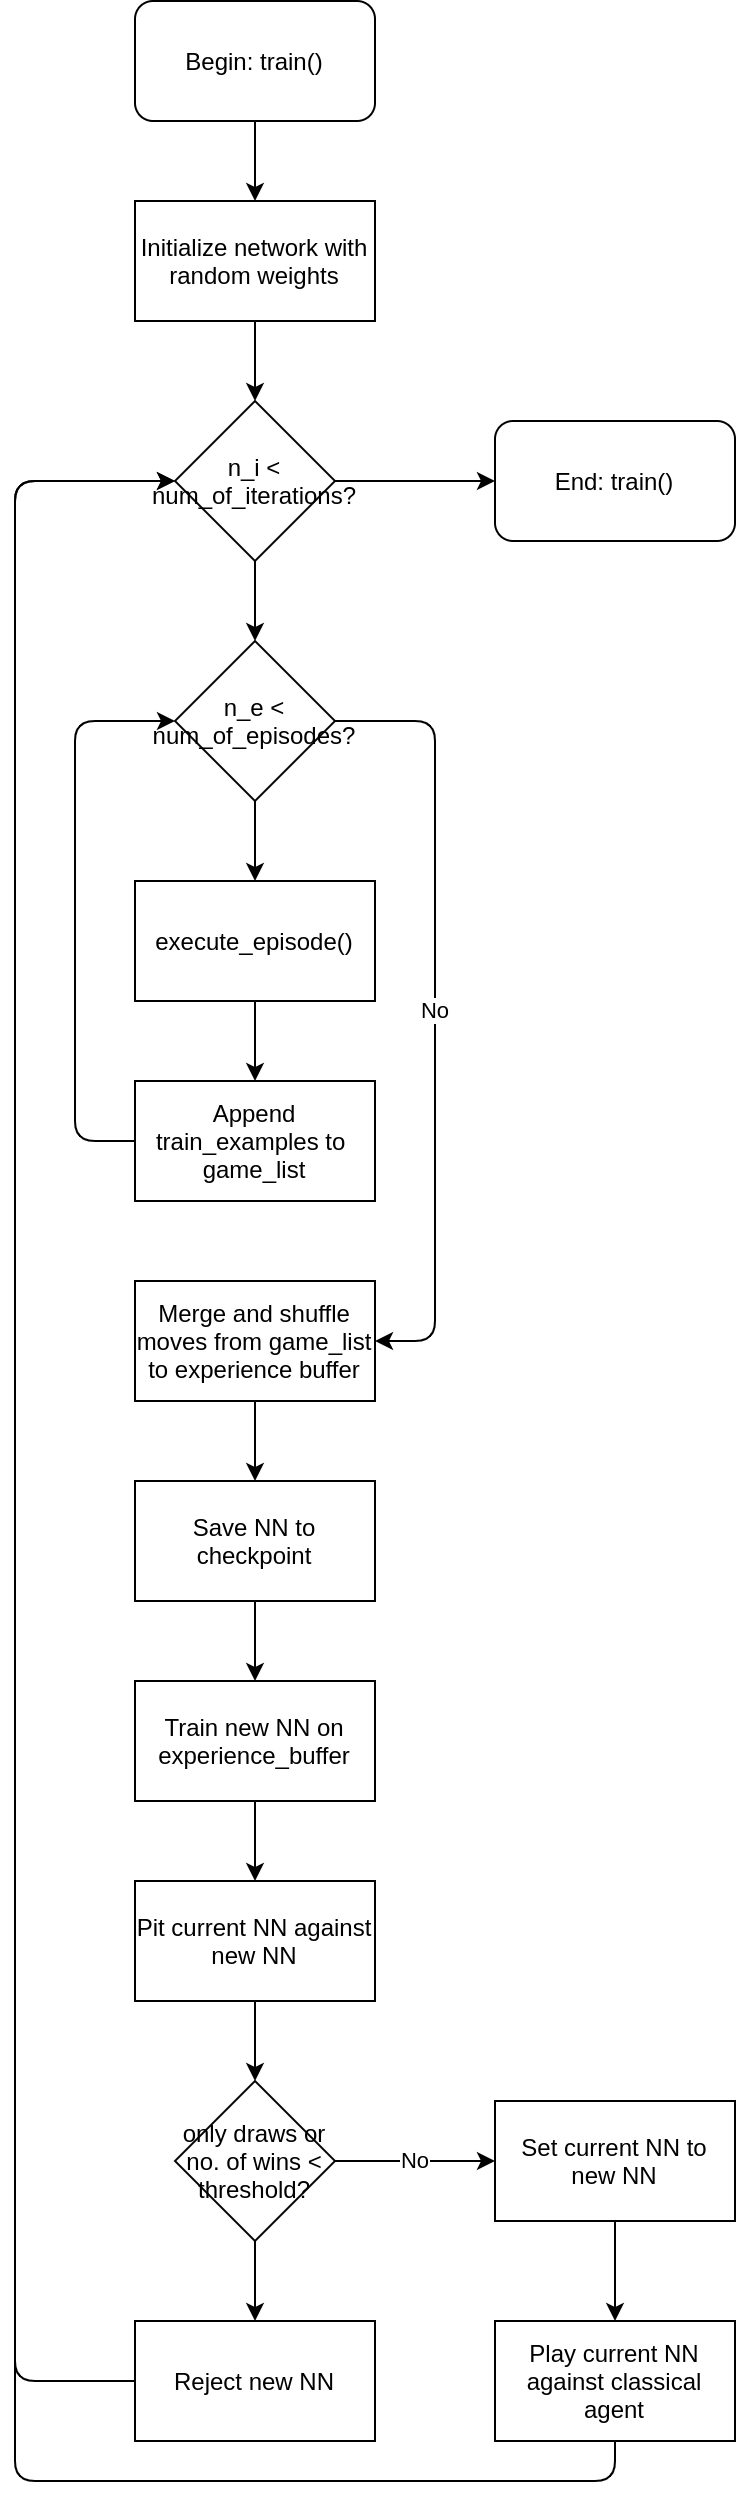
\includegraphics[height=19cm, keepaspectratio]{training_main_loop.png}
    }
    % \hfill
    \subfloat[The episode loop]{
        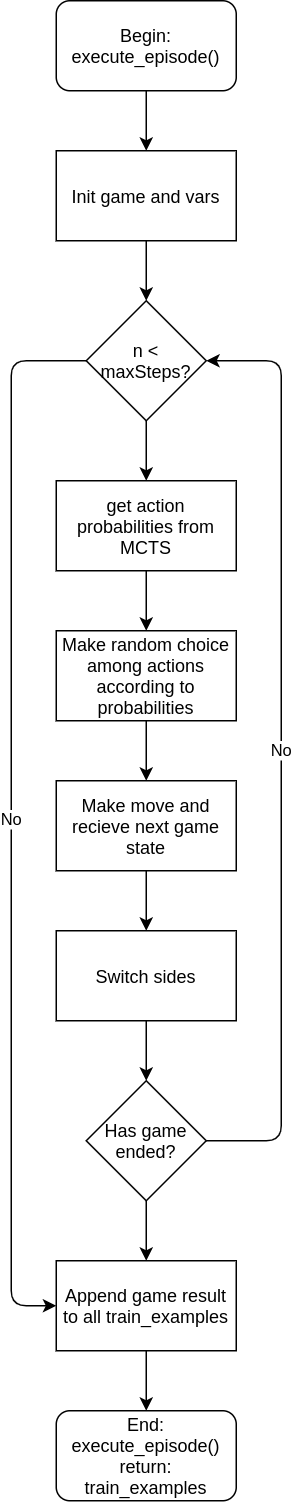
\includegraphics[height=19cm, keepaspectratio]{training_episode.png}
    }
    \caption{The self-play training pipeline}
    \label{training_algorithm}
\end{figure}

\subsection{Parallelization}
\label{parallelization}
AlphaZero General's training pipeline does not offer parallel training. By comparing the time taken to execute one episode for the game of Othello and Abalone, it showed that a game of Abalone takes on average $40$ times (n=100) longer to finish: 1s for Othello and 40s for Abalone. Investigating potential improvements, it became clear that two major factors determine the runtime of an episode:

1. Length of the game. A game of Abalone takes significantly more turns, caused by rules not forbidding loops such that games can be infinite. Moreover, defensive play styles can draw out games significantly. In order to alleviate the issue, we limited the number of turns $m$ per game. In this case, the length was limited to $m=200$. The newly created terminal state is scored with a partial score: The scored marbles are subtracted by the opponent's score for each player. We scored win or loss as either $1$ or $-1$. Hence, the partial score is normalized by the number of marbles needed to win. The partial score reflects which player had the upper hand at the artificial terminal state.

2. The MCTS being computationally expensive: A closer inspection of the execution time, holding all variables constant, demonstrates the culprit. The simulation step of MCTS uses the neural network. The time taken by this function is one order of magnitude larger than the second most expensive operation, which is the generation of legal moves. For example, when running 15 MCTS iterations with the original TensorFlow implementation, one turn takes

\begin{itemize}
    \item Total time: 0.44s
    \item One MCTS iteration: 0.03s
    \item Neural network : 0.025s
    \item Valid move generation: 0.05s
\end{itemize}

Looking at the main variables that control the length of the nested loops, it becomes clear that reducing the time an MCTS iteration takes is essential. Assuming function $f$ is the operation to perform one Monte Carlo simulation:

$$
    k := \text{number of games}
$$
$$
    m := \text{number of turns per game}
$$
$$
    n := \text{number of MCTS simulations}
$$
$$
    f \in O(kmn)
$$

Abalone requires a larger number of MCTS simulations. The other projects \cite{bruasdal_deep_2020,thakoor_learning_nodate} used only 30 iterations for Othello and Hex, but Abalone has a much more complex game tree. AlphaZero performs $1,600$ iterations \cite[p. 11]{silver_mastering_2017} for each move. The MCTS needs to recommend a better move than the pure network to improve. It is the policy improvement operator. Those properties were the reason to decide to use PyTorch. The library brings a $5$-times improvement for that step as shown in \ref{pytorch_vs_tensorflow_performance}. Nevertheless, this only brings down execution time for one episode by a factor of $5$, still being $8$-times slower than the reference implementation for Othello. AlphaZero uses two ways to alleviate this problem:

\begin{itemize}
    \item Parallelization of the self-play training
    \item Parallelization of the MCTS (APV-MCTS)
\end{itemize}

As Python's global interpreter lock \cite{noauthor_globalinterpreterlock_nodate} does not allow for true multithreading. Parallelizing the MCTS poses significant complexity and difficulty. However, allowing for simultaneous self-play and neural network training is feasible. As already mentioned in section \ref{training_framework}, the implementation by Bruåsdal \cite{bruasdal_deep_2020} provides this feature. For that reason, its architecture is used as a blueprint for migrating AlphaZero General into a parallel architecture. The figure \ref{parallel_training_pipeline} depicts how the components mentioned interacting in a parallel fashion.

\begin{figure}[H]
    \centering
    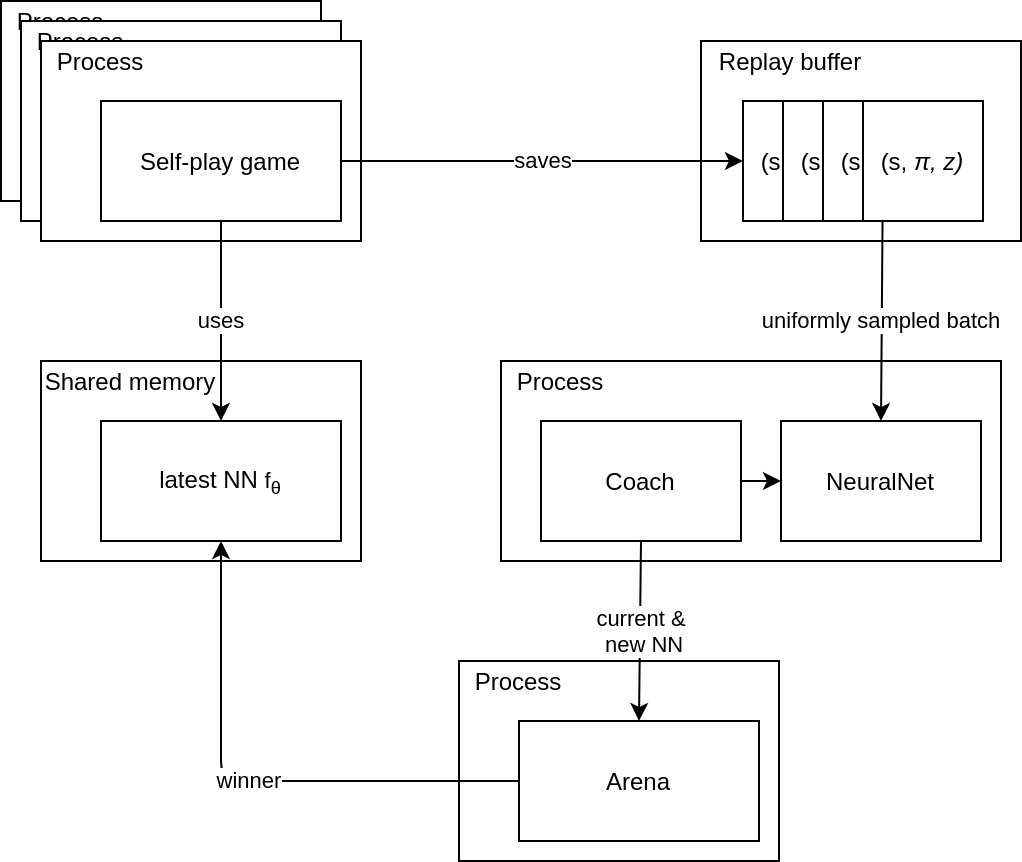
\includegraphics[height=10cm, keepaspectratio]{parallel-training.png}
    \caption{The different processes during the parallel training \cite[cf. p. 45]{bruasdal_deep_2020}}
    \label{parallel_training_pipeline}
\end{figure}

The self-play workers use the current best neural network $f_{\theta}$ to generate experience. The experience is put into a queue to allow for asynchronous communication between the worker processes and the Coach. The queue is emptied and loaded into the replay buffer for each neural network training iteration. If the experience buffer exceeds the maximum size, the oldest experience is dropped. The number of training batches is defined by the batch size and buffer size (buffer size divided by batch size). The training batches are created by randomly sampling tuples ($s, \pi, z$) from the buffer. No tuple is used twice so that the entire buffer is utilized.

After training the neural network with the batches, the newly created network is pitted against the old version in the Arena. As both variants have to be pitted against each other multiple times, we parallelized the Arena. If the new network is stronger than the previous version, it is saved on disk. Then the version counter is incremented. The version counter is a shared variable between the workers and the Coach. After each completed self-play game, the worker checks if the version counter is larger than its stored version. If that is the case, the new network is loaded from disk.

An important factor is to balance the number of workers against the time it takes to train the neural network. If the buffer grows large, training takes a long time. In the meantime, much new experience is potentially generated, overriding all previous experience. As a result, all experience is only generated from one network. The training process might become less robust.

\subsection{Distribution}
The table \ref{pytorch_vs_tensorflow_performance} shows the usage of a GPU accelerates the inference speed significantly, particularly for PyTorch. Ergo, accelerating the self-play is highly desireable. When multiple processes utilize a GPU, each process requires a portion of the cards memory. PyTorch has the feature to share a model between multiple processes, wherefore a model does not need to be fully loaded for each process \cite{noauthor_module_nodate}. However, in PyTorch "every-time a process holds any pytorch object that is allocated on the GPU, then it allocates an individual copy of all the kernels (cuda functions) that pytorch uses, which is about 1GB" \cite{radim_shark_sharing_2020}. We observed that an unshared model uses 1.2GB of VRAM per process and decided to not to use the memory-sharing feature. The additional overhead to implement it did not justify the saved memory. Each process loads its own instance of the model.

Either way at some point the worker's VRAM needs outgrows the GPU's resources. We implemented the parallelization in such a way, that the user can assign GPU identifiers to each component (arena, training loop and workers). The processes then distribute the processes equally to the given hardware.

\subsection{Symmetrical Board Generation}
Abalone's board has six rotational symmetries and six mirror axes, as mentioned in \ref{state_space_complexity}. By generating the symmetrical board states for each tuple ($s, \pi, z)$, the data can be augmented by a factor of twelve. That means $\pi$ and $v$ are equivalent for up to 12 symmetrical board states. Some board configurations have less symmetrical boards, as some are identical. For example, rotating the default starting position by 120° produces the same board as mirroring it by the $s$ axis. In general, the factor of 12 does hold for almost all board states.

The first step in generating the symmetrical boards is to turn the marble positions into cube coordinates. There is a simple way for cube coordinates to mirror and rotate coordinates. A mapping function transforms marble coordinates from their matrix coordinates of the form $(x, y)$ to $(q, r, s)$. The origin of the cube coordinate system is laid into the center of the Abalone board, such that e.g. $E5 = (0, 0, 0)$ or $A1 = (-4, 4, 0)$.

The transformed coordinates can be rotated around the origin by 60° clockwise by shifting the values to the right and negating the values:

\begin{BVerbatim}
    [ q,  r,  s ]
    to  [-r, -s, -q ]
    to     [  s,  q,  r ]
\end{BVerbatim}

To mirror a cube coordinate along one of the three main coordinate axes $q, r$ or $s$ the two coordinates that don't belong to the axis are swapped:

\begin{BVerbatim}
    function reflect_q(h) { return Cube(h.q, h.s, h.r); }
    function reflect_r(h) { return Cube(h.s, h.r, h.q); }
    function reflect_s(h) { return Cube(h.r, h.q, h.s); }
\end{BVerbatim}

The coordinates need to be negated first for mirroring along the orthogonal axis to the main axis. Besides all marbles, all moves in $\pi$, whose probability is not $0$, have to be transformed as well. First, the move corresponding to the index in $\pi$ is looked up. As a move consists of one or two marble coordinates, those are transformed by the same scheme. The directions can be transformed into cube coordinates as well:

\begin{BVerbatim}
    (+1, -1, 0): NORTH_EAST
    (+1, 0, -1): EAST
    (0, +1, -1): SOUTH_EAST
    (-1, +1, 0): SOUTH_WEST
    (-1, 0, +1): WEST
    (0, -1, +1): NORTH_WEST
\end{BVerbatim}

This way, the same functions can be applied to the directions. After all operations are applied, the cube coordinates are converted back to marble coordinates and moves. In the case of the moves, the probabilities from the original $\pi$ are written to the new index position.

\subsection{Warm-Up}
AlphaZero starts learning from scratch. Thus, there is no information about what constitutes a good move or strategy. The result is a cold-start problem. The self-play learning might not improve performance or even harm performance for an extended period of time. Equipped with ample computational resources like DeepMind, this poses no problem and is even desirable: The network is not nudged into a specific direction and can produce more novel insights.

Investigations into the application of AlphaZero's training principle showed possible ways to warm-start the training of the network \cite{wang_adaptive_2021}. Wang proposes an adaptive rollout-based warm-start. The method reintroduces rollouts into the MCTS that are performed at the beginning of the training process and are slowly phased out over the course of training.

Another possibility would be to reintroduce components of AlphaGo. Either by using a database of moves or letting the agent train against a heuristic agent. For Abalone, we propose a similar method. By letting a heuristic agent play against a random agent, an initial experience buffer is created. Thus, the first iteration of the training of $f_{\theta}$ produces a function that approximates the heuristic player. We hypothesized that the self-play further improves this warmed-up agent like it did in the RL step in AlphaGo.

\chapter{Experiments and Results}
\label{experiments-and-results}

Each experiment has a hypothesis, a setup, and a result.

\section{Hardware}
For the purpose of this thesis, we had access to two machines. The smaller machine is a personal machine, and the large machine is rented at the provider Exoscale \cite{noauthor_exoscale_nodate}. They will be referred to as \textit{Balthazar} and \textit{Melchior} respectively. Their specifications are described in table \ref{hardware}. \textit{Caspar} was a larger version of Melchior, but the additional GPU was not useful. Therefore Caspar is not considered further.

\begin{table*}[!h]
    \begin{center}
        \begin{tabular}{ c|c|c }
            Component & Balthazar             & Melchior                \\
            \hline
            \hline
            CPU       & 6 Core AMD Ryzen 3600 & 24 Core Intel Broadwell \\
            RAM       & 32GB                  & 120GB                   \\
            GPU       & NVIDIA GTX 1660 Super & 3 $\cdot$ NVIDIA P100   \\
            VRAM      & 6GB                   & 3 $\cdot$ 16GB          \\
            Storage   & 500GB SSD             & 400GB SSD               \\
        \end{tabular}
    \end{center}
    \caption{Hardware specifications of the utilized machines}
    \label{hardware}
\end{table*}

\section{Parameters}
\label{parameters}
A multitude of parameters controls the behavior of the system. The most relevant hyperparameters are listed in table \ref{parameters}. If one of the parameters differs from the default values in an experiment, it will be mentioned. For each experiment, all parameters are persisted by the system.

\begin{table}
    \begin{center}
        \begin{tabularx}{\textwidth}{ c|c|X }
            Name                       & Default   & Explanation                                                                                   \\
            \hline
            \hline
            temp\_treshhold            & 60        & The number of moves for which the next move is sampled (cf. equation \ref{eq:move_selection}) \\
            update\_treshold           & 0.6       & The percentage of matches, that has to be won for a new network to be accepted                \\
            num\_MCTS\_sims            & 120       & The number of times the search tree is expanded during MCTS                                   \\
            num\_self\_play\_workers   & 9         & The number of workers used for parallel self-play                                             \\
            num\_arena\_workers        & 8         & The number of workers used for parallel Arena matches                                         \\
            load\_model                & false     & Indicates whether to load an existing model                                                   \\
            maxlen\_experience\_buffer & 1,000,000 & The maximum number of tuples ($s, \pi, z$) in the buffer                                      \\
            nnet\_size                 & mini      & The neural net used as introduced in \ref{neural_network_architecture}                        \\
            lr                         & 0.001     & The learning rate during training of the neural network                                       \\
            epochs                     & 10        & The number of of epochs during training of the neural network                                 \\
            batch\_size                & 64        & The size of the batches during training of the neural network                                 \\
        \end{tabularx}
    \end{center}
    \caption{The parameters of the training pipeline}
    \label{parameter_table}
\end{table}

\section{Validation}
\paragraph{Hypothesis} The modified framework still converges to optimal play for TicTacToe and Othello.
\paragraph{Setup} Run pipeline with modified implemenation of TicTacToe and Othello from \cite{thakoor_suragnairalpha-zero-general_nodate} on Balthazar.

\begin{table}[!h]
    \begin{center}
        \begin{tabular}{ c|c }
            Name                       & Value   \\
            \hline
            \hline
            temp\_treshhold            & 15      \\
            num\_MCTS\_sims            & 30      \\
            num\_self\_play\_workers   & 2       \\
            num\_arena\_workers        & 2       \\
            maxlen\_experience\_buffer & 960,000 \\
        \end{tabular}
    \end{center}
    \caption{The parameters for the naive run}
\end{table}

\paragraph{Result} Convergence to optimal play for TicTacToe (cf. figure \ref{tictactoe_performance}) and Othello very likely.

\begin{figure}[!h]
    \centering
    \subfloat[TicTacToe $3 \cdot 3$ field]{
        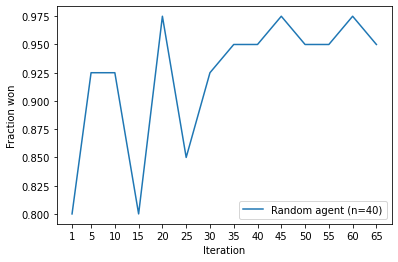
\includegraphics[height=5cm, keepaspectratio]{validation_tictactoe.png}
    }
    \hfill
    \subfloat[Othello $6 \cdot 6$ field]{
        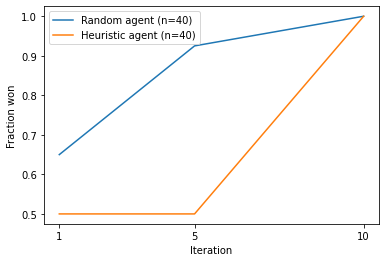
\includegraphics[height=5cm, keepaspectratio]{validation_othello.png}
    }
    \caption{Win-ratio against random baseline in TicTacToe and Othello. Win-ratio is $\frac{\text{gamesWon}}{\text{allGames}}$ }
    \label{tictactoe_performance}
\end{figure}

\section{Application}
\subsection{Naive Run}
\paragraph{Hypothesis} The naive implementation without any Abalone specific modifications converges to optimal play.
\paragraph{Setup} Run pipeline on Balthazar.

\begin{table}[!h]
    \begin{center}
        \begin{tabular}{ c|c }
            Name                       & Value   \\
            \hline
            \hline
            num\_MCTS\_sims            & 60      \\
            num\_self\_play\_workers   & 2       \\
            num\_arena\_workers        & 2       \\
            maxlen\_experience\_buffer & 960,000 \\
        \end{tabular}
    \end{center}
    \caption{The parameters for the naive run on Balthazar}
\end{table}

\paragraph{Result} No improvement in playing performance, cf. figure \ref{performance_local_naive}
\begin{figure}[!h]
    \centering
    \subfloat[The win-ratio]{
        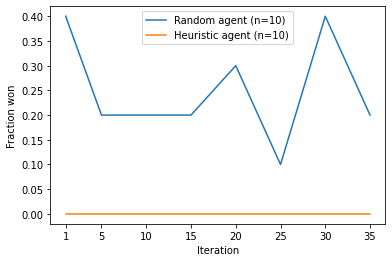
\includegraphics[height=5cm, keepaspectratio]{performance_local_win_ratio.png}
    }
    \hfill
    \subfloat[The cumulative reward]{
        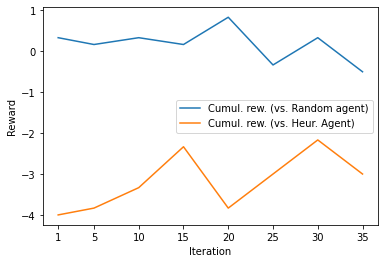
\includegraphics[height=5cm, keepaspectratio]{performance_local_reward.png}
    }
    \caption{The training performance for the naive run}
    \label{performance_local_naive}
\end{figure}

\subsection{Naive Run with large NN}
\paragraph{Hypothesis} The naive implementation without any Abalone specific modifications converges to optimal play with the large NN.
\paragraph{Setup} Run pipeline on Balthazar.

\begin{table}[!h]
    \begin{center}
        \begin{tabular}{ c|c }
            Name                       & Value   \\
            \hline
            \hline
            num\_MCTS\_sims            & 60      \\
            num\_self\_play\_workers   & 2       \\
            num\_arena\_workers        & 2       \\
            maxlen\_experience\_buffer & 960,000 \\
            nnet\_size                 & large   \\
        \end{tabular}
    \end{center}
    \caption{The parameters for the naive run on Balthazar}
\end{table}

\paragraph{Result} No improvement in playing performance, cf. figure \ref{performance_local_naive_large}. The network seems to have a bug leading to strong divergence. We decided to discard the implementation for the time being as the inference and training of the network took approximately 30\% longer.
\begin{figure}[!h]
    \centering
    \subfloat[The win-ratio]{
        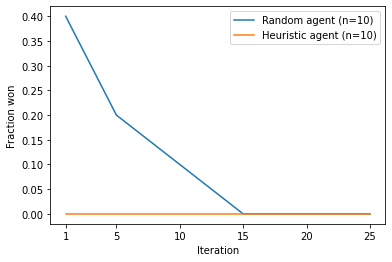
\includegraphics[height=5cm, keepaspectratio]{performance_local_naive_large_win_ratio.png}
    }
    \hfill
    \subfloat[The cumulative reward]{
        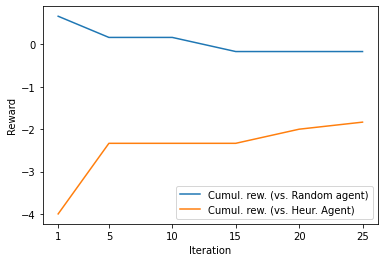
\includegraphics[height=5cm, keepaspectratio]{performance_local_naive_large_cumul_reward.png}
    }
    \caption{The training performance for the naive run with the large NN}
    \label{performance_local_naive_large}
\end{figure}

\subsection{Scaled naive Run}
\paragraph{Hypothesis} The naive implementation without any Abalone specific modifications converges to optimal play on a larger machine with a bigger buffer and more workers.
\paragraph{Setup} Run pipeline on Melchior.
\paragraph{Result} No improvement in playing performance, divergence, cf. figure \ref{performance_remote_naive}
\begin{figure}[!h]
    \centering
    \subfloat[The win-ratio]{
        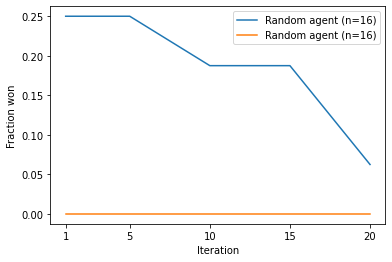
\includegraphics[height=5cm, keepaspectratio]{performance_remote_naive_win_ratio.png}
    }
    \hfill
    \subfloat[The cumulative reward]{
        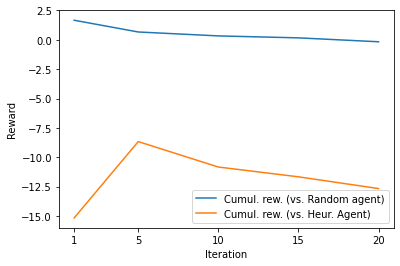
\includegraphics[height=5cm, keepaspectratio]{performance_remote_naive_reward.png}
    }
    \caption{The training performance for the scaled naive run}
    \label{performance_remote_naive}
\end{figure}

\subsection{Reward Distribution}
\paragraph{Hypothesis} The distribution of game results $z$ is uneven.
\paragraph{Setup} Plot histogram of $z$ in experience buffer of the previous run.
\paragraph{Result} Most of the games end up as drawn or with minor advantage for one player, cf. figure \ref{distribution_of_rewards}).

\begin{figure}[!h]
    \centering
    \subfloat[The experience buffer after the fifth iteration]{
        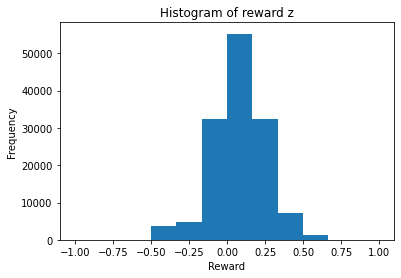
\includegraphics[height=5cm, keepaspectratio]{performance_local_exp_buffer_5.png}
    }
    \hfill
    \subfloat[The experience buffer after the twentieth iteration]{
        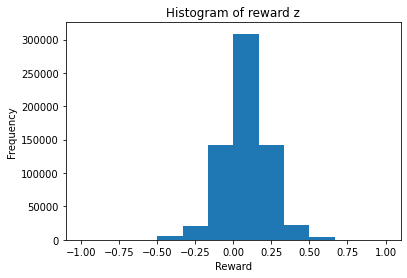
\includegraphics[height=5cm, keepaspectratio]{performance_local_exp_buffer_20.png}
    }
    \caption{Distribution of $z$ in experience buffer of the naive run on Balthazar.}
    \label{distribution_of_rewards}
\end{figure}

\subsection{Scaled warmed-up Run}
\paragraph{Hypothesis} Warming the network up with experience generated by Verloop's minimax against a random player nudges the network towards more aggressive play. The resulting experience buffer has stronger signals $z$, which improves performance.

\paragraph{Setup} Run pipeline on Melchior with a warmed-up network.

\begin{table}[!h]
    \begin{center}
        \begin{tabular}{ c|c }
            Name        & Value \\
            \hline
            \hline
            load\_model & true  \\
        \end{tabular}
    \end{center}
    \caption{The parameters for the validation runs}
\end{table}

\paragraph{Result} The agent maintains its strength against the random agent throughout the training. The performance against the heuristic agent begins to improve. About half of the games are drawn and the marble losses incurred decrease, cf. figure \ref{performance_remote_warmed_up}. However, during 16 iterations only four new networks were accepted. The rate of acceptance decreases over time. The experience buffer during different iterations of the training run looks promising. The distribution shows much higher rewards, many games even ending before the cutoff of 200 moves, cf. figure \ref{performance_remote_warmed_up_exp_buffer}. Nevertheless, there seems to be a trend of the rewards to gravitate towards more draws.

\begin{figure}[!h]
    \centering
    \subfloat[The win-ratio]{
        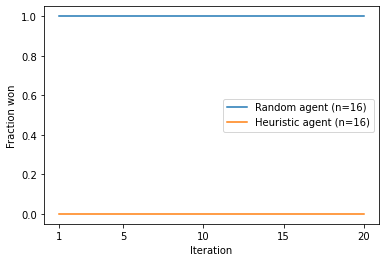
\includegraphics[height=5cm, keepaspectratio]{performance_remote_warmed_win_ratio.png}
    }
    \hfill
    \subfloat[The cumulative reward]{
        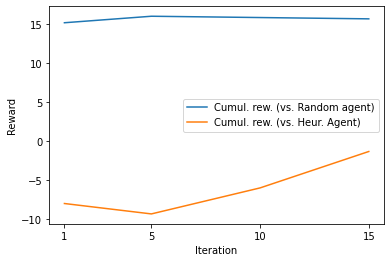
\includegraphics[height=5cm, keepaspectratio]{performance_remote_warmed_cumul_reward.png}
    }
    \caption{The training performance for the scaled warmed-up run}
    \label{performance_remote_warmed_up}
\end{figure}

\begin{figure}[!h]
    \centering
    \subfloat[The experience buffer after the first iteration]{
        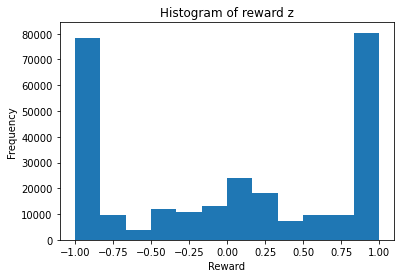
\includegraphics[height=5cm, keepaspectratio]{performance_remote_warmed_up_exp_buffer_1.png}
    }
    \hfill
    \subfloat[The experience buffer after the tenth iteration]{
        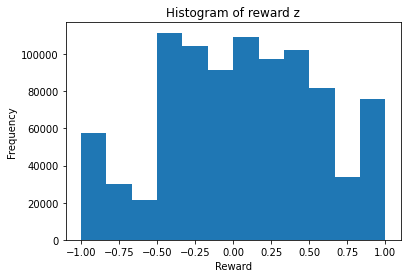
\includegraphics[height=5cm, keepaspectratio]{performance_remote_warmed_up_exp_buffer_10.png}
    }
    \hfill
    \subfloat[The experience buffer after the fifteenth iteration]{
        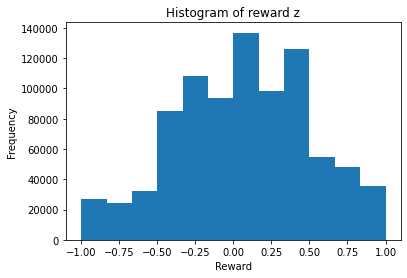
\includegraphics[height=5cm, keepaspectratio]{performance_remote_warmed_up_exp_buffer_15.png}
    }
    \caption{Initially the buffer is still filled with the experience from the prewarming phase, where all games ended with eiter -1 or 1 reward.}
    \label{performance_remote_warmed_up_exp_buffer}
\end{figure}

\begin{figure}[!h]
    \centering
    \subfloat[The agent shows strong play, drawing against the heuristic agent]{
        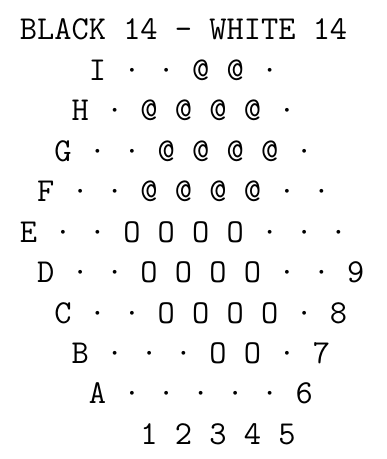
\includegraphics[height=5cm, keepaspectratio]{warmed_up_net_strong_play.png}
    }
    \subfloat[The agent shows weak play, loosing formation and getting pressed against the brink of the board]{
        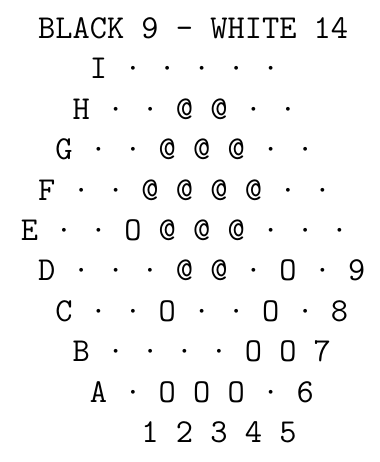
\includegraphics[height=5cm, keepaspectratio]{warmed_up_net_weak_play.png}
    }
    \caption{The final board positions against heuristic player, during training iteration 10 with the warmed up NN}
    \label{performance_remote_warmed_up_heuristic}
\end{figure}

\subsection{Scaled Run with adjusted Reward}
\paragraph{Hypothesis} The reward function provides no penalty for long matches, that result in a draw.
\paragraph{Setup} Run pipeline on Melchior with adjusted reward function. Each turn has a reward of $-0.001$, for a maximum game length of 200 that is a maximum of $-0.2$. The other rewards remain unchanged.

\paragraph{Result} Inconclusive for the amount of iterations performed. A tendency of improvement is present.
\begin{figure}[!h]
    \centering
    \subfloat[The win-ratio]{
        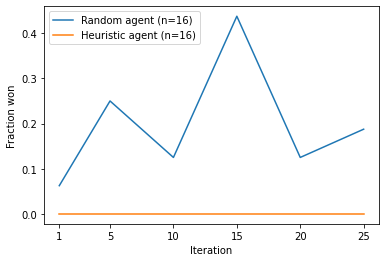
\includegraphics[height=5cm, keepaspectratio]{performance_remote_diff_z_win_ratio.png}
    }
    \hfill
    \subfloat[The cumulative reward]{
        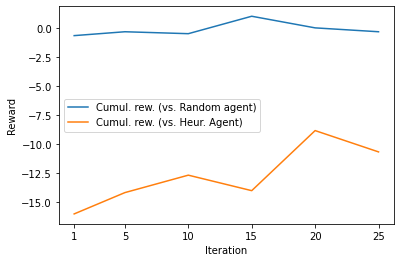
\includegraphics[height=5cm, keepaspectratio]{performance_remote_diff_z_cumul_reward.png}
    }
    \caption{The training performance for the scaled run with adjusted reward}
    \label{performance_remote_diff_z}
\end{figure}

\subsection{Runtime of Experiments}
\paragraph{Hypothesis} The training of the neural network has become a bottleneck.
\paragraph{Setup} Compare lengths of training iterations on Balthazar and Melchior.

\paragraph{Result} Due to the parallel nature, self-play games are generated continuously. The longer one training iteration takes, the bigger the backlog of new games becomes. One iteration took, on average, one h. The training of the network has become the limiting factor, not the generation of self-play games, cf. figure \ref{iteration_duration}. The serialized experience buffer (with Python pickle) with 1,000,000 items takes 10GB of storage. As the entire buffer is used for training, a long training duration is to be expected.

\begin{figure}[!h]
    \centering
    \subfloat[Training run on Balthazar]{
        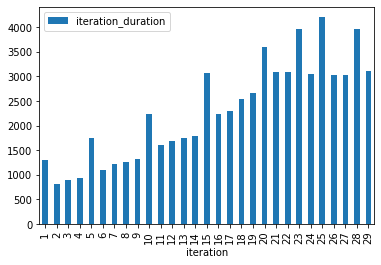
\includegraphics[height=5.2cm, keepaspectratio]{performance_local_iteration_duration.png}
    }
    \hfill
    \subfloat[Training run on Melchior]{
        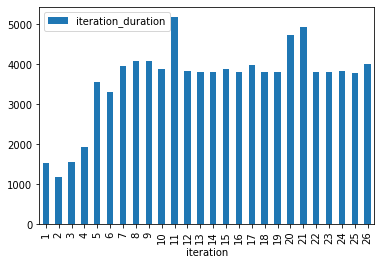
\includegraphics[height=5.2cm, keepaspectratio]{performance_remote_naive_iteration_duration.png}
    }
    \caption{Duration of one training iteration in seconds. The training times stabilize once the experience buffer has reached its maximum size.}
    \label{iteration_duration}
\end{figure}
\chapter{Conclusion}
\label{conclusion}
The method proposed by AlphaZero is extremely powerful and has proven to be promising for Abalone as well. Due to limitations in compute for the experiments it has not been possible to replicate the ground breaking success achieved in Go for Abalone. This also points at the major downside of the method as it requires significantly more compute than any classical knowledge based methods. Gradient descent and even simple feedfowards for neural networks are very expensive operations even with the proliferation of ever more powerful hardware accelerators. The hardware used by DeepMind for AlphaGo is only accessible to top researchers in the field due to the high cost. There are two main potential avenues through which we could reap the benefits of this method with lower capital requirements:

\begin{itemize}
    \item Further theoretic improvements bringing significant speedups. This could be something along the lines of the incremental improvement between AlphaGo and AlphaZero or full paradigm shifts in the methodology.
    \item The cost for training neural networks coming down by an order of magnitude from current levels. This could be due simply to the passage of time as in the past accelerators like GPUs still followed an exponential improvementrate as observed in Moore's Law for CPUs \cite{moore_cramming_2006} ("Huang's Law" \cite{noauthor_huangs_2021}). Another factor would be archtitectural changes that improve scalability and performance for deep learning specifically. Additionally, the rising economic significance of machine learning has provided an incentive for more specialized hardware like TPUs \cite{noauthor_tpu_nodate} or Jim Keller's Grayskull. \cite{noauthor_grayskull_nodate} The same reason reignited interest in optical computing accelerators to bring drastic changes in power requirements and performance for matrix multiplication. \cite{noauthor_lightmatter_nodate,noauthor_lightelligence_nodate}
\end{itemize}

\bibliographystyle{../lib/IEEEtran}
\bibliography{ref}

\end{document}
